% !TEX TS-program = pdflatex
% !TEX encoding = UTF-8 Unicode

%tells you if you use obsolete packages
%\RequirePackage[l2tabu,orthodox]{nag}

\documentclass[]{article}

\usepackage[utf8]{inputenc} % set input encoding (not needed with XeLaTeX)
\usepackage[T1]{fontenc}

\DeclareUnicodeCharacter{00A0}{ }

%%% PAGE DIMENSIONS
\usepackage{geometry} % to change the page dimensions
\geometry{a4paper} % or letterpaper (US) or a5paper or....
\geometry{margin=2.5cm}
% \geometry{landscape} % set up the page for landscape
%   read geometry.pdf for detailed page layout information

\usepackage{graphicx} % support the \includegraphics command and options

% \usepackage[parfill]{parskip} % Activate to begin paragraphs with an empty line rather than an indent

%%% PACKAGES
\usepackage{booktabs} % for much better looking tables
\usepackage{array} % for better arrays (eg matrices) in maths
\usepackage{paralist} % very flexible & customisable lists (eg. enumerate/itemize, etc.)
\usepackage{verbatim} % adds environment for commenting out blocks of text & for better verbatim
\usepackage{subfig} % make it possible to include more than one captioned figure/table in a single float
\usepackage{listings} %for code listings
\usepackage{color} %for colored syntax highligting
\usepackage{rotating}
\usepackage{pdflscape}
\usepackage[]{algorithm2e}
\usepackage{multirow}
\usepackage{float}
\usepackage{mathtools}
\usepackage{amssymb}



\usepackage{caption}
% \captionsetup[subfigure]{format=subfig,labelsep=colon,labelformat=simple}
% \usepackage{subcaption}

\usepackage[backend=bibtex, bibencoding=utf8]{biblatex}
\bibliography{biblib} 
%%% Code listing
\definecolor{mygreen}{rgb}{0,0.6,0}
\definecolor{mygray}{rgb}{0.5,0.5,0.5}
\definecolor{mymauve}{rgb}{0.58,0,0.82}
\lstset{
basicstyle=\footnotesize\ttfamily,
commentstyle=\color{mygreen},
keywordstyle=\color{blue},
numberstyle=\tiny\color{mygray},
numbers=left,
tabsize=2,
frame=tb,
aboveskip=3mm,
belowskip=3mm,
breaklines=true,
breakatwhitespace=true,
showstringspaces=false,
columns=flexible
}

% to include a file as a listing: \lstinputlisting{intio.c}
% inline listing: \begin{lstlisting}[frame=single]

%%% HEADERS & FOOTERS
\usepackage{fancyhdr} % This should be set AFTER setting up the page geometry
\pagestyle{fancy} % options: empty , plain , fancy
\renewcommand{\headrulewidth}{0pt} % customise the layout...
\lhead{}\chead{}\rhead{}
\lfoot{}\cfoot{\thepage}\rfoot{}

%%% ToC (table of contents) APPEARANCE
\usepackage[nottoc,notlof,notlot]{tocbibind} % Put the bibliography in the ToC
% \usepackage[titles,subfigure]{tocloft} % Alter the style of the Table of Contents
%\renewcommand{\cftsecfont}{\rmfamily\mdseries\upshape}
%\renewcommand{\cftsecpagefont}{\rmfamily\mdseries\upshape} % No bold!
\usepackage{hyperref} % use hyperlinked ToC
\hypersetup{colorlinks=true, linkcolor=black, citecolor=black, filecolor=black, urlcolor=black}
\graphicspath{ {ImageLib/} }

\usepackage[printonlyused]{acronym}

%%%-------------------------------------------------------------------


\title{Third Year Group Project \\ State Estimation for Indoor Environments}
\author{Oskar Weigl, Ryan Savitski, Thomas Morrison, Chinemelu Ezeh, Joshua Elsdon}
\begin{document}
\maketitle
\center{\textbf{\large{\emph{"I think we will have it flying by tonight..."}	}}}


%\center{\textbf{\large{\emph{"...a profound trust in the advances of science."}	}}}

\abstract{
This report investigates the design of indoor state estimation techniques, and demonstrates one particular implementation using a depth camera mounted to a quadcopter frame. The approach consists of collecting data from the environment and detecting planes within it. Using these in combination with an extended Kalman filter we estimate the location of the frame. We combine more traditional sensors such as an accelerometer and gyro to complete the localisation system. We investigate the hardware necessary to process point clouds in real time. Further to this we propose a calibration algorithm for the Xtion Pro depth camera and demonstrate its success.   
\tableofcontents


%\section{Acronyms} % (fold)
%\label{sec:acronyms}
\begin{acronym}
	\acro{DBScan}{Density Based Spatial Clustering of Applications with Noise}
	\acro{DoF}{Degrees of Freedom}
	\acro{EKF}{Extended Kalman Filter}
	\acro{GPS}{Global Positioning System}
	\acro{IMU}{Inertial Measurement Unit}
	\acro{ISA}{Instruction Set Architecture}
	\acro{MAV}{Micro Aerial Vehicle}
	\acro{MMSE}{Minimum mean square error}
	\acro{PCA}{Principle component analysis}
	\acro{PCL}{Point Cloud Library}
	\acro{RANSAC}{Random Sample Consensus}
	\acro{RGB-D}{Red Green Blue - Depth}
	\acro{RGB}{Red Green Blue}
	\acro{SLAM}{simultaneous localization and mapping}
	\acro{UAV}{Unmanned Aerial Vehicle}
	\acro{ToF}{time of flight}
\end{acronym}
%\clearpage
% section acronyms (end)

\section{Executive Summary} % (fold)
\label{sec:executive_summary}
\subsection{Introduction}
%todo: Ryan: imo rewrite quite a lot of exec sum
%todo: exec sum should be at the front? separate doc?
In the present world of increasing machine presence and autonomy, it is important for robots to be able to correctly and accurately estimate their position, velocity and in general their current state. This project focused on determining the state of flying robots in GPS denied environments, this first step towards implementing indoor SLAM. With this in mind, we served as consultants to a start up company called Mavrx who specialises in developing UAVs, supporting electronics and software platforms. Our mission is to enhance MAVRX's  research by developing an indoor state estimator that can be used for autonomous quadcopters, whist keeping the system portable to other kinds of airframe.
\subsection{Our Solution}
The proposed solution the indoor localisation problem consists of using the Xtion Pro depth camera to track planar surfaces in the environment for absolute positioning. This type of feature is somewhat simple to extract and robust to changes in view point, further to this walls ceilings and floors all are ubiquitous within man made environments. These planes will be used in conjunction with inertial sensors with an extended Kalman filter to provide an optimal estimation of our state that is resilient to noise. This system was implemented on an Intel Atom x86 board that has a mini-itx form factor.


%We propose a solution targeting indoor environments which consists of using on-board processing with an inexpensive RGB-D camera as our primary sensor combined with accelerometer and gyroscope sensors capable of working in GPS denied areas. Our approach leverages the powerful yet cheap capabilities of the Xtion Pro camera. A typical solution to localisation involves modelling the motion of the agent as it moves in the environment, extracting features from the environment using sensors and then combining this information to approximate its location within the environment. We decided to track planes (i.e. walls) as our features, extracting plane equations from the Xtion Pro using intelligent vision algorithms with good resistance to noise and bounded-time operation. Moreover, using an RGB-D camera provides a plethora of information and resilience to interference compared to that of sonar or infra-red sensors. For the state estimation engine, we employ the widely popular Kalman filter as it produces optimal solutions in the presence of noise.  
\subsection{Results}
Using vision algorithms, we were able to extract planes as features. Observing three orthogonal planes provides full observability in the x, y and z axes. Using the extended Kalman filter, we were able to show that our system can estimate its position, velocity and attitude in an indoor environment. We had to tune the filter providing empirical values for uncertainties in the Xtion's observation obtained through numerous testing. We confirmed the consistency of our filter by checking for bias in its measurement error and ensuring its bounds is described by its covariance. Our system gave us reliable positioning, within 10mm accuracy. Unfortunately due to hardware limitations introducing large amounts of delay into the control loop the system can no longer be stable without large initial oscillations. Further to this the small viewing angle of the Xtion made maintaining a view on an appropriate number of planes difficult and the inertial sensors are high enough quality to maintain an accurate state in between plane observations. 

\subsection{Conclusion}
Localisation and state estimation is a first step towards full autonomous simultaneous localisation and mapping which combined with the high maneuverability of a quadcopter opens up new domains in robotic applications. We have thus pushed forward the goal of our client company, Mavrx, in developing unmanned aerial vehicles. Our project has shown and demonstrated the possibilities of indoor state estimation without GPS data which has commercial benefits in the aerial photography market as well as applications in search and rescue operations. Our system can be applied in the industry where aerial monitoring is essential such as pipeline inspection and area mapping.  


\clearpage


\section{Problem Specification}
\label{sec:problem_specification}

\subsection{Context} % (fold)
\label{sub:context}

There are often situations where unmanned aerial vehicles (UAVs) are useful, including: search and rescue, infrastructure inspection, videography and military applications such as reconnaissance. These tasks are already performed routinely by UAVs, though usually controlled remotely by a human operator. In some cases the human operator is removed, and Global Positioning System (GPS) is used to close the loop on absolute positioning. This is a functional solution, as it is quite cheap and can work nearly anywhere in the world. However, there are also places where GPS will not work reliably, such as inside a building or between many tall buildings (often called an urban canyon). These environments also would put pressure on the skill of a human operator due to the abundance of obstacles.
Therefore there is increased interest in autonomous micro aerial vehicles (MAVs) that can operate in such GPS denied environments.

% subsection context (end)

\subsection{Project Aim}
\label{sub:what_are_we_trying_to_achieve}
This project aims to build a functional prototype of an indoor state estimation algorithm that can operate in GPS denied environments, such as indoors and in urban canyons. The aim of the prototype is to be a proof of concept, showing that the above is possible with current, off the shelf technology. Also the state estimation system will be trialled on a quadcopter airframe to demonstrate its function and investigate its properties and usefulness for micro aerial vehicles. 

\subsection{Who are Mavrx and why are they interested?} % (fold)
\label{sub:why_are_mavrx_interested_in_this_work_}

Mavrx is a small start-up firm that is aiming to provide autonomous aerial imaging hardware and software for commercial enterprise. Additionally, Mavrx has a daughter firm, UAir, that targets the hobbyist market and which recently succeeded in crowd-funding a cheap quadcopter development platform. They have asked us to help develop a indoor state estimation system, such that a fully autonomous flying platform can be created to operate indoors. The system should be priced in the consumer range rather than the military/commercial category of existing platforms. Mavrx are not particularly interested in in depth pricing or business analysis, so most of the emphasis of this report will be on implementation and testing. 


\subsection{Related research} % (fold)
\label{sub:related_works}
The approaches to localisation for UAVs in GPS denied environments fall into three main categories: optical flow tracking \cite{DBLP:conf/icra/GrabeBG12}, time of flight (ToF) laser scanners \cite{Bry2012} and colour with depth (RGB-D) cameras \cite{Shen2012}.

Grabe et al. \cite{DBLP:conf/icra/GrabeBG12} produced a MAV that uses a downward facing RGB camera on a quadcopter to correct for sensor drift. This approach's highlight is the low cost of hardware, as cheap RGB cameras are now common place in many consumer electronics. In combination with other cheap sensors such as gyroscopes, accelerometers, magnetometers and barometers, a complete navigation solution becomes easily affordable. The downsides of this approach include no easy way to extract absolute data from the system. The concept of an absolute distance must be derived from the inertial sensors at some point, hence the whole system could be susceptible to drift over time. The conclusion of this paper suggests that this system would be well applied as a backup for a more robust tracking system. Therefore we can dismiss the use of optical flow tracking as a primary localisation technique. 

Bry et al. \cite{Bry2012} use a fixed-wing model aircraft and a planar time of flight range finder for their localisation scheme. The use of a fixed-wing aircraft offers one main advantage: efficiency, enabling longer flight times compared to rotary aircraft such as helicopters and quadcopters. The drawback is that a fixed wing aircraft must be continually moving in order to stay airborne, and hence is more restricted in confined environments. The ToF range finder is a very promising technology for localisation as it provides accurate data at high update rates. Hovewer, the technology is also expensive, with the authors of the aforementioned work using a device priced at \$5600.
%http://www.acroname.com/robotics/parts/R314-HOKUYO-LASER4.html)

As such, laser scanner sensors are out of the project's target solution price. Furthermore, these range finders only scan in one plane, hence returning quite sparse data. In order to identify features one must accumulate data along many planes, which, depending on feature type, may make detection time prohibitively long. 

Shen et al. \cite{Shen2012} use a quadcopter airframe and a RGB-D camera combined with a laser range finder for localisation. Using the depth channel of the camera they extract point cloud data to form an occupancy map and localise using the laser scanner. The benefit of the RGB-D camera is that due to this technology being pushed to entertainment platforms, the sensors are now considerably cheaper than before (e.g. Microsoft's Kinect at \$200). 
%todo: need to tie this up in a better way
%todo: given time, add the gaussian pyramid optical slam from IARC 2010(ish) entry.


% % section problem_specification (end)
\section{Implementation Overview}
\label{sub:implementation_overview}

% dropped below:
% Our state estimator involves a moving agent such as a quadcopter which deploys one sensor to gather information about its surroundings. This is called an exteroceptive sensor and in our case, we use a depth camera. We also incorporate extra sensors to measure the agent's own movement. These are called preprioceptive sensors and we used an accelerometer and a gyroscope. The state evaluation process involves the following steps:


% \textbf{The agent moves, reaching a new point of view in the room} As a result of unavoidable noise
% and errors, this movement increases the uncertainty on the robot's localization.
% There is a need to model this motion to in implementing our state evaluation. This, we will call the motion model.
	
% \textbf{The robot observes features in the room which need to be added to its interior map.} These features we call called landmarks. However, dues to errors in the depth camera, the location of the landmark will be uncertain. Moreover the robot's already uncertain position means that these two uncertainties have to be properly combined. We thus require a mathematical model to determine the position of the landmark from data obtained by the exteroceptive sensor. This we will call the inverse observation model.

% \textbf{The robot re-observes landmarks and it uses them to  make corrections to its self-localisation and landmark position.} Thus reducing uncertainties on both. We also need a mathematical model to predict the values of the measurement from the predicted landmark location and the robot localisation. This will be the direct observation model.

% The tasks can be group into two main categories feature extraction and extended Kalman filter implementation.

The primary sensor for the implementation is consumer grade depth camera, in this case the Xtion pro. This camera will view the environment and output a point cloud, which is a quantised representation of the space in 3D, these are captured at 30 frames per second with a resolution of 160x120. Then using the Point Cloud Library (PCL) all large planes are extracted by, first, finding local normals at each point are computed using integral images \cite{Holz2011} and then clustering them using a custom Flood Fill algorithm.  The use of integral images lets us remove the high frequency noise from the depth camera in a computationally efficient manner. At this stage there is a point cloud in xyz space with a local normal vector $(N_x, N_y, N_z)$ at each point. 

The custom Flood Fill algorithm starts with a set of randomised seed points within the CCD pixel space (as each pixel corresponds to a point in xyz space). For each seed, the fill incrementally grows a cluster by visiting neighbours along the CCD (i.e. xy) space. The condition for adding a point to the cluster is derived from how similar the local normal is at that point to that of the initial seed. Clusters are then rejected if they do not meet the depth-dependent minimum parameter, the clusters passing this test are considered further as planar patches. The feature extraction pipeline also calculates the uncertainties associated with the discovered planes, passing that information to the EKF. An alternative clustering approach, based on the DBScan algorithm was also evaluated and is discussed in the relevant section. These planes and the data from the accelerometer, gyro and sonar sensor are sent to the Extended Kalman Filter (EKF). 

%The localisation scheme used is based on a feature tracking Extended Kalman Filter (EKF).The filter fuses all the sensors sensors: accelerometer; gyroscope; downward facing sonar and  with which in turns allows the quadrotor to localise itself within the environment. The features tracked are planar surfaces within the environment, which are obtained from depth data of a consumer RGB-D camera.The depth camera of choise is the Asus Xtion Pro as it is considerably lighter than the copeting products, while maintaining a similar price point. Due to the relatively narrow field of view (58$^{\circ}$ horizontal, 45$^{\circ}$ vertical), the floor and the ceiling is expected to often be out of view, resulting in reduced observability in the elevation direction. The depth camera is complemented with a downward facing sonar sensor to address this issue. Planes are tracked as they can represent walls, floors and ceiling, which are abundant in man-made environments, are static and easily reobservable. Furthermore, this abstraction drastically reduces both the computational and space complexity of the filter. 

The job of the EKF is to perform an optimal evaluation of the robot's state given the presence of uncertainties in measurements. The EKF is a non-linear extension of the Kalman filter which is itself a linear quadratic estimator capable of giving optimal values of a measurement in the presence of noise. Its results are more accurate than those obtained from single measurements. The EKF operates iteratively producing optimal values around the current mean and covariance. The other alternative to the EKF is the particle filter. The main difference is that the EKF produces optimal results using an approximate mathematical model while the particle filter produces optimal results based on physical models.
Based on a comparative study \cite{CompareFilters} on the difference between the two approaches, for Gaussian noise model the Kalman filter will always produce a better result in less computation time.

The state of the robot consists of its position, velocity, attitude, accelerometer and gyroscope biases, and landmark positions. The non-trivial state components, the biases due to temperature variation and manufacturing process errors, are stored because they exhibit a random walk and thus depend on their previous values. The Kalman filter iteratively updates the robot's state along with its uncertainties, referred to as its covariance matrix.

% The feature extraction pipeline starts with 160x120 depth frames at 30 frames per second from the RGB-D camera. Using Point Cloud Library (PCL) the data is transformed into a xyz point cloud. Next, local surface normals at each point are computed using integral images \cite{Holz2011}. The use of integral images lets us remove the high frequency noise from the depth camera in a computationally efficient manner. At this stage there is a point cloud in xyz space with a local normal vector $(N_x, N_y, N_z)$ at each point. 

% The above point cloud is then clustered by a custom Flood Fill algorithm.

Incoming plane data invokes an update iteration in the EKF, which tries to associate measured planes to existing features in its state. The association is based on Mahalanobis distance, which is a measurement used in multi-dimensional statistical analysis for classification of samples.

Additionally, the project produced the necessary mathematical derivations and a partial implementation of feature registration. Registration enables the filter to increase the landmark map with previously unobserved features online. This will allow the quadrotor to solve the full simultaneous localisation and mapping (SLAM) problem and operate in environments without any prior knowledge.

The aircraft configuration of choice is a quadcopter for our demonstration platform, due to its ability to navigate environments with limited space and stability. The latter also helps to reduce the amount of motion blur in the depth camera. Finally, it presents a good opportunity to test Mavrx/UAir's R10 quadcopter platform's reliability and robustness.


\section{Preliminaries}

\subsection{System platform} % (fold)
\label{sub:system_platform}

The project aims to implement the estimation algorithm on on-board processing, this section discusses the hardware platform for the implementation.

In conventional processor applications, of importance is optimising the computational performance against cost and power usage. For an embedded system that is mounted on a quadcopter however, power usage of the chip is not a concern as it is insignificant compared to the usage of the MAV itself. Therefore, for implementing this project we desire the best processing power per pound for the target workload. In this metric, no distinct advantage can be given to either of the two main standard processor architecture families (x86 and ARM) and the evaluation needs to be done on a chip-by-chip basis. 

In addition to the above, the choice of the instruction set architecture is influenced by the architecture's operating system support and the ability to interface with other system components that could be incorporated into the system (e.g. coprocessors). The target operating system for this project is a lightweight distribution based on the Linux kernel. This is due to the Linux kernel being free, open source and being easily configurable, with the ability to compile in only the needed functionality and put options in loadable kernel modules. This results in an embedded operating system with minimal memory and processing footprint, as well as small disk usage which can be limited in embedded systems. For the specific libraries and frameworks used in implementing the estimation software (PCL and OpenNI), x86-Linux variants were found to have more mature support than ARM-Linux at the time of writing.

For low volume production, it is not always worth investing the engineering time in designing a custom hardware platform, sourcing the components and manufacturing. Instead, small form factor boards can be readily purchased at acceptable prices. For example: \$90 Odroid-U2 development board with a quad core ARM Cortex-A9 @1.7 GHz processor with a Mali-400 quad core GPU in a 60x60x60 mm package.

Additionally, we evaluated the possibility of using consumer grade smartphones as the embedded processing platform for the estimation algorithm. Android mobile operating system is built on top of the Linux kernel and is also open source, making it the OS of choice for this evaluation. The reasons for considering consumer grade smartphones are as follows:

\begin{itemize}
	\item the smartphone market is extremely competitive, driving the prices down while improving the processing power to levels compatible with embedded systems usually seen in robotics applications.
	\item small form factor, lack of need for additional heatsinks.
	\item smartphones of all price ranges come with additional hardware and sensors that can be useful for the quadcopter platform. Most devices have 9 degree of freedom (DoF) sensors and USB functionality, making it possible to interface with the RGB-D camera. Additionally, the estimation can be improved by using the phone's camera in a downwards looking configuration as an optical flow sensor \cite{DBLP:conf/icra/GrabeBG12}. GPS can be used in semi-indoor environments and urban canyon situations. Wifi can be used to augment the system with wifi-slam \cite{Wifi-slam} for additional localisation information in indoor environments. Furthermore, GPUs found in smartphones are starting to be OpenCL compatible (e.g. Imagination Technologies' powerVR series and newer ARM Mali cores), which can provide easily accessible acceleration for certain parts of the algorithm.
\end{itemize}

However, in practice it was found that porting third party libraries used in the project and drivers for the RGB-D camera sensor, while possible, needed significant investment of engineering time. Additionally, the android platform enforces restricted APIs to underlying hardware resources, so it is not always possible to get the direct hardware control (e.g. for the intertial measurement unit) usually found in embedded Linux systems.

For the above reasons, the project was implemented on Intel Atom D2550 (Dual Core @1.86 GHz) processor running x86-Linux. 

%extra possibility: throw in fpga as additional possibilities?, zynq7 style?, fixed point scaling etc


\subsection{Sensor Calibration} % (fold)

The depth data obtained by the RGB-D camera of choice has two distinct adverse properties. Firstly, the depth values are quantised to levels that scale quadratically, i.e. there is a loss of resolution at longer distances. Feature extraction needs to account for this effect and have depth-dependent parameters. Secondly, the factory calibration of the sensor was evaluated and found to be inadequate for our application, already seeing as much as 23.5\% error at 4 meter distance. This section further discusses the sensor's performance and our calibration routine.

Additionally, it is important to note that transforming per-pixel depth data to a xyz point cloud is based on the cone projection model of the sensor. Therefore an error in the depth measurement for a pixel will also introduce error in the corresponding point's x and y coordinates within the xyz space.
%todo: paint a quick and dirty explanation picture?

As mentioned above, the factory calibration of the RGB-D camera's depth sensor is unsatisfactory for the target application. Straight walls as seen by the sensor at distances of more than 2m quickly become warped (see example in Figure~\ref{fig:uncal5m2}). Such depth data quality would make robust feature extraction infeasible at distances of interest.


\begin{figure}[htb]
\centering     %%% not \center
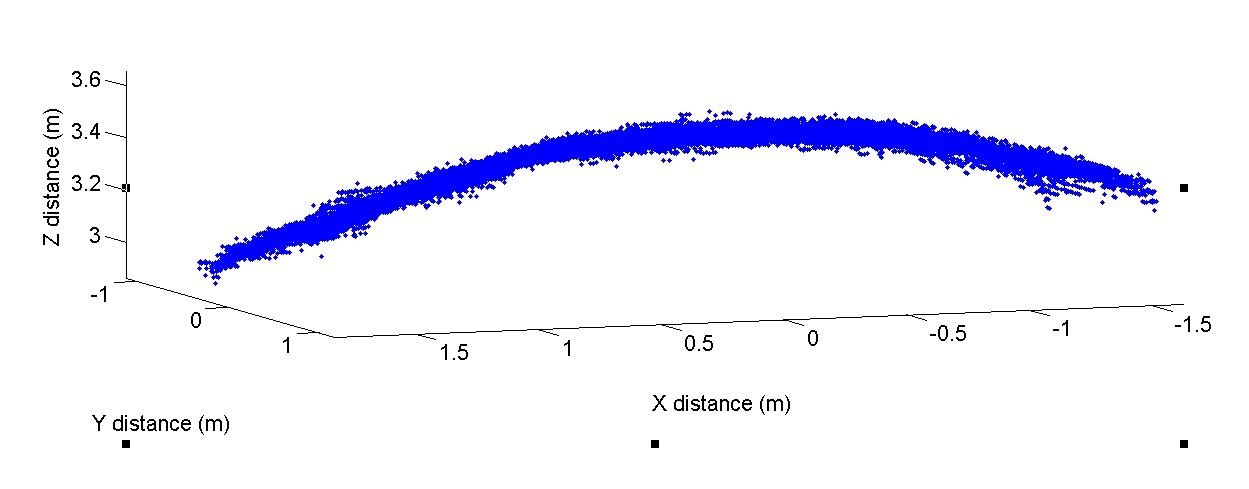
\includegraphics[width=0.8\textwidth]{uncal5m2.PNG}
%\subfloat[coloured point cloud]{\label{fig:clouduncal5m}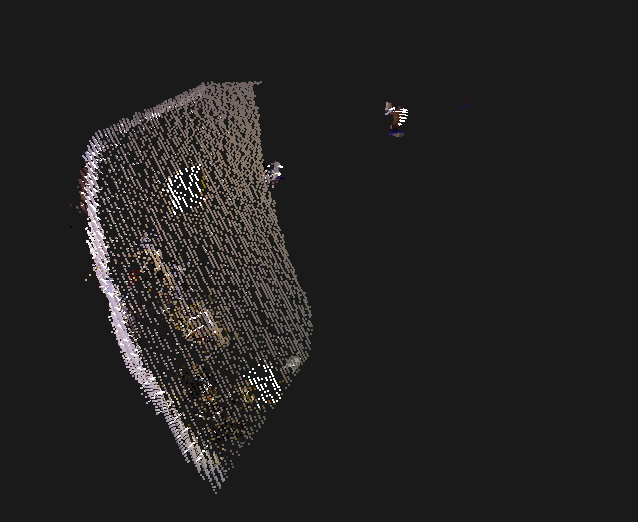
\includegraphics[width=60mm]{wallat6m}}
\caption{Example of the poor factory calibration of the Xtion sensor when looking at a wall 4 meters from the camera, plotted as xyz space point cloud.}
\label{fig:uncal5m2}
\end{figure}

Figure~\ref{fig:avDist2} shows the average depth across a frame capture for a planar surface as measured at a range of distances. It can be seen that the depth data is not just warped per pixel, but also wrong on average. For example, at 4m the average distance measured was 3.32m, which represents a 17\% error. The maximum per-pixel error being 0.941m at 4m, which corresponds to 23.5\% error. 

\begin{figure}[htb]
	\begin{center}
		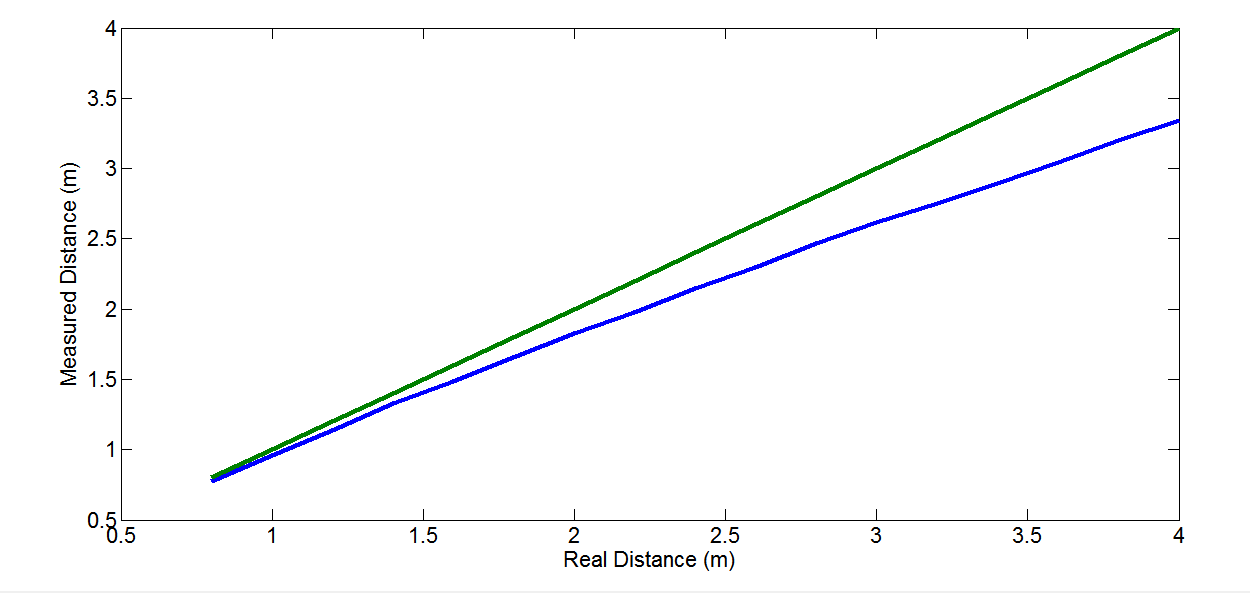
\includegraphics[width = 0.8\textwidth]{avDist2}
	\end{center}
	\caption{Measured distance against true distance as average of all the pixels per frame. Measured data in blue. Ground truth in green.}
	\label{fig:avDist2}
\end{figure}

Given the paired measurement and ground truth data, we mapped the correction vectors into a 3D space that can be looked up to correct new data. In order to have the 3D correction field be continuous, data needs to be smoothed and interpolated in all 3 dimensions. One significant issue is that all obtained correction vectors fall into thin regions in the 3D space along the camera-z (i.e. depth) axis, and within those areas the data is dense in the x and y dimensions. Therefore our task is to preform smoothing in the x and y directions to remove the signal noise and to find a good interpolation scheme looking in the camera-z direction.  

In order to avoid large computation times on the embedded device it is important that the correction function is inverted to a map from measured to corrected data. Otherwise, for each data point in the input, it would be required to search for the two closest calibration measurements for that pixel. With an inverted correction lookup table it is possible to go directly to the correct entries in the table (i.e. in $O(1)$). Assuming the uninverted approach doing binary search, this accounts for a factor of 3 difference at the depth data compensation stage. 

\subsection{Results of calibration} % (fold)
 \label{sub:results_of_calibration}
 After performing the calculations described above we are left with 19200 look up tables (one for each CCD pixel), each of these contain the real depth value for a given depth measurement. Figure~\ref{fig:beforeAfter} shows an example of the depth data before and after correction for one given distance test, where both images are produced by subtracting the frame's average depth from all pixels and setting the dynamic range to be from -10\% of the average to +10\%. Therefore an ideal image of a plane would be of pure grey. Table~\ref{tab:averages} shows the average distance measured over the whole plane for a range of measurements and their respective corrections, it can be seen that both the local and global inaccuracies have been effectively compensated. 

 Figure~\ref{fig:outputTest} visualises the importance of the calibration. The camera took the data points while pointing at a flat wall, a small section of orthogonal flat wall is also in view. With only the factory calibration, the walls are curved and the data points describing them are dispersed, including an error in average depth. After processing, the walls are properly orthogonal and flat. Furthermore, the grouping of the data points to the surface is much better.


\begin{figure}[htb]
	\centering     %%% not \center
	\subfloat[Before correction]{\label{fig:preflat8}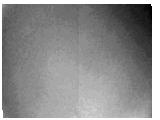
\includegraphics[width=60mm]{preflat8}} \;
	\subfloat[After correction]{\label{fig:postflat8}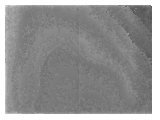
\includegraphics[width=60mm]{postflat8}}
	\caption{Example of the correction function in action for a flat surface at a specific distance from the sensor. Images show divergence from the measurements average distance, white is +10\% and black is -10\% of the average respectively.}
	\label{fig:beforeAfter}
\end{figure}
\begin{figure}[htb]
	\centering     %%% not \center
	\subfloat[Before processing]{\label{fig:NewBeforeMatlab}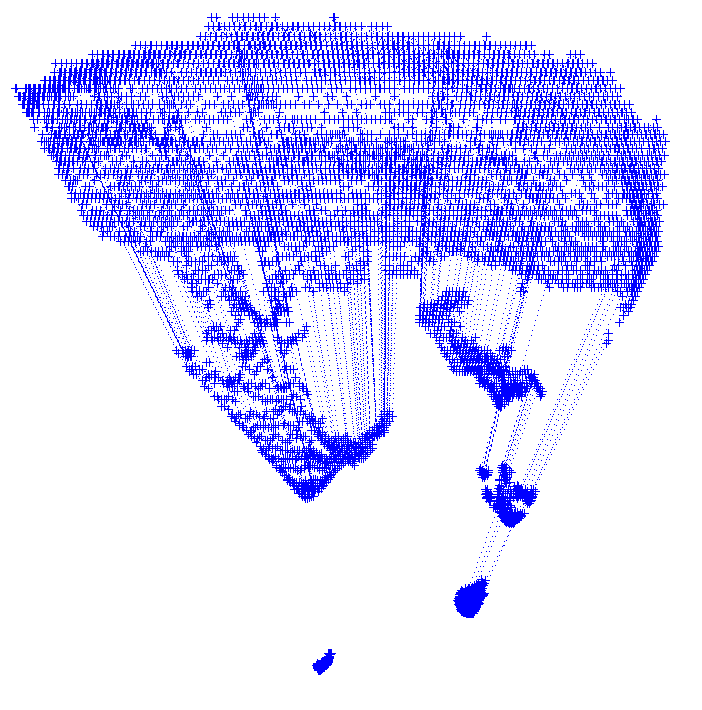
\includegraphics[width=60mm]{NewBeforeMatlab2.PNG}} \;
	\subfloat[After processing]{\label{fig:NewAfterMatlab}\includegraphics[width=60mm]{NewAfterMatlab2}}
	\caption{A demonstration of the correction compensating for the systematic depth errors. Plotted as a projection of xyz point cloud data.}
	\label{fig:outputTest}
\end{figure}

\begin{figure}[htb]
	\begin{center}
	\begin{tabular}{ccc}
		\hline

		\hline
		\textbf{Set Distance}& \textbf{Measured Distance}& \textbf{Corrected Distance} \\
		\hline
		0.8		& 0.773	& 0.800\\
		1.0		& 0.960	& 1.002\\
		1.2 	& 1.138	& 1.201\\
		1.6 	& 1.483	& 1.601\\
		1.8 	& 1.655	& 1.800\\
		2.0 	& 1.826	& 2.001\\
		2.2 	& 1.976	& 2.186\\
		2.4 	& 2.146	& 2.415\\
		2.6 	& 2.299	& 2.590\\
		2.8 	& 2.465	& 2.804\\
		3.0 	& 2.614	& 2.988\\
		3.2 	& 2.751	& 3.158\\
		3.4 	& 2.895	& 3.370\\
		3.6 	& 3.045	& 3.591\\
		3.8 	& 3.198	& 3.815\\
		4.0 	& 3.341	& 3.993\\
		\hline

		\hline
	\end{tabular}
	\end{center}
	\caption{Average distance measured over the whole plane for a range of measurements and their respective corrections, all units in meters.}
	\label{tab:averages}
\end{figure}


 % subsection results_of_calibration (end) 
\clearpage


\section{Feature Extraction} % (fold)
\label{sec:feature_extraction}

The feature extraction pipeline aims to identify and classify planar surfaces within the data coming from a forward facing depth camera, the reasoning for extracting planes is given in section \ref{sub:implementation_overview}. The input data is depth values for 160x120 pixel frames at 30 fps, which is turned into a point cloud using the Point Cloud Library (PCL). Local surface normals are found at each point, which are used for clustering the data into planar patches with a flood fill algorithm. The details of each stage in the feature extraction are presented in this section. 

Two clustering algorithms were designed, implemented and evaluated: a density based scan (DBScan) variant and a flood fill algorithm, with the final implementation using the latter.
\subsection{Normal Estimation} % (fold)
\label{sub:normal_estimation}

As the depth sensor is a consumer grade RGB-D camera, operated at over double the quoted distance, the depth data is significantly noisy. A naive local surface normal kernel would take several nearest neighbours to a point and construct its local normal. However, with the high frequency noise level seen in the sensor readings, this method would produce effectively random normals. Instead, we use a technique called integral image convolution \cite{Holz2011} to combine normal estimation with low pass filtering. This is done through a data structure called an integral image (also known as a summed area table), which is computationally efficient and allows the normal estimator to run in real time. 

The downside of low pass filtering is illustrated in Figure~\ref{fig:spurious_plane_normals}, which shows that intersections of planes (which are common indoors) are smoothed and instead look like curved surfaces. This can cause clustering algorithms to either follow the smooth curve and classify everything as one cluster, or instead break the curve into many planar strips. This problem was one of the main concerns and is discussed further in the clustering algorithms' sections. Additionally, the kernel nature of the normal estimator effectively reduces the depth sensor's field of view as it cannot operate on points near edges. Furthermore, the sensor cannot return data around sharp depth discontinuities due to parallax. This means that the kernel operator is also unable to operate within very small clusters of points. The kernel's size used in this prototype was the experimentally best tradeoff between low pass filtering of noise, corruption of edges and reduction of the sensor's field of view.

\begin{figure}[p]
	\centering     %%% not \center
	\subfloat[Smoothed corners can give rise to planar strips being found by plane finding algorithms]{
		\label{fig:spurious_plane_normals1}
		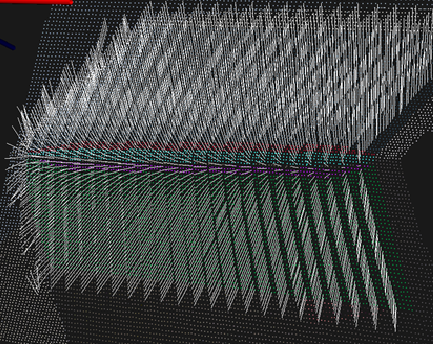
\includegraphics[width=0.4\textwidth]{6spuriousplanes_normals.PNG}
	}
	\;
	\subfloat[high frequency content along the edge of two orthogonal planes smoothed by the kernel]{
		\label{fig:spurious_plane_normals_2}
		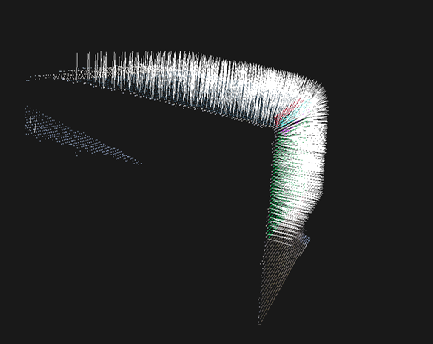
\includegraphics[width=0.4\textwidth]{6spuriousplanes_normals_2.PNG}
	}

	\caption{Effects of the low pass filtering by the normal estimation kernel}
	\label{fig:spurious_plane_normals}
\end{figure}

\subsection{Density Based Scan} % (fold)
\label{sub:density_based_scan}


One popular algorithm for density based clustering is density based scan (DBScan), which can find arbitrarily shaped clusters, needs no apriori cluster count information and a has a notion of noise. The basic idea is to take an initial point and find all other neighbouring points within a certain neighbourhood (of a distance $\epsilon$). If enough are found (decided by a threshold value $\gamma$), then these neighbouring points are iteratively expanded upon, again checking if the minimum number of neighbouring points ($\gamma$) is sufficient to be considered within the same cluster. Figure~\ref{fig:dbscan} demonstrates a pass of the algorithm starting from a point within region A and clustering outward until the density of connected points becomes too small. Listing~\ref{alg:dbscan} details the full algorithm to find all densely connected regions within an image space.

\begin{figure}[bt]
	\begin{center}
		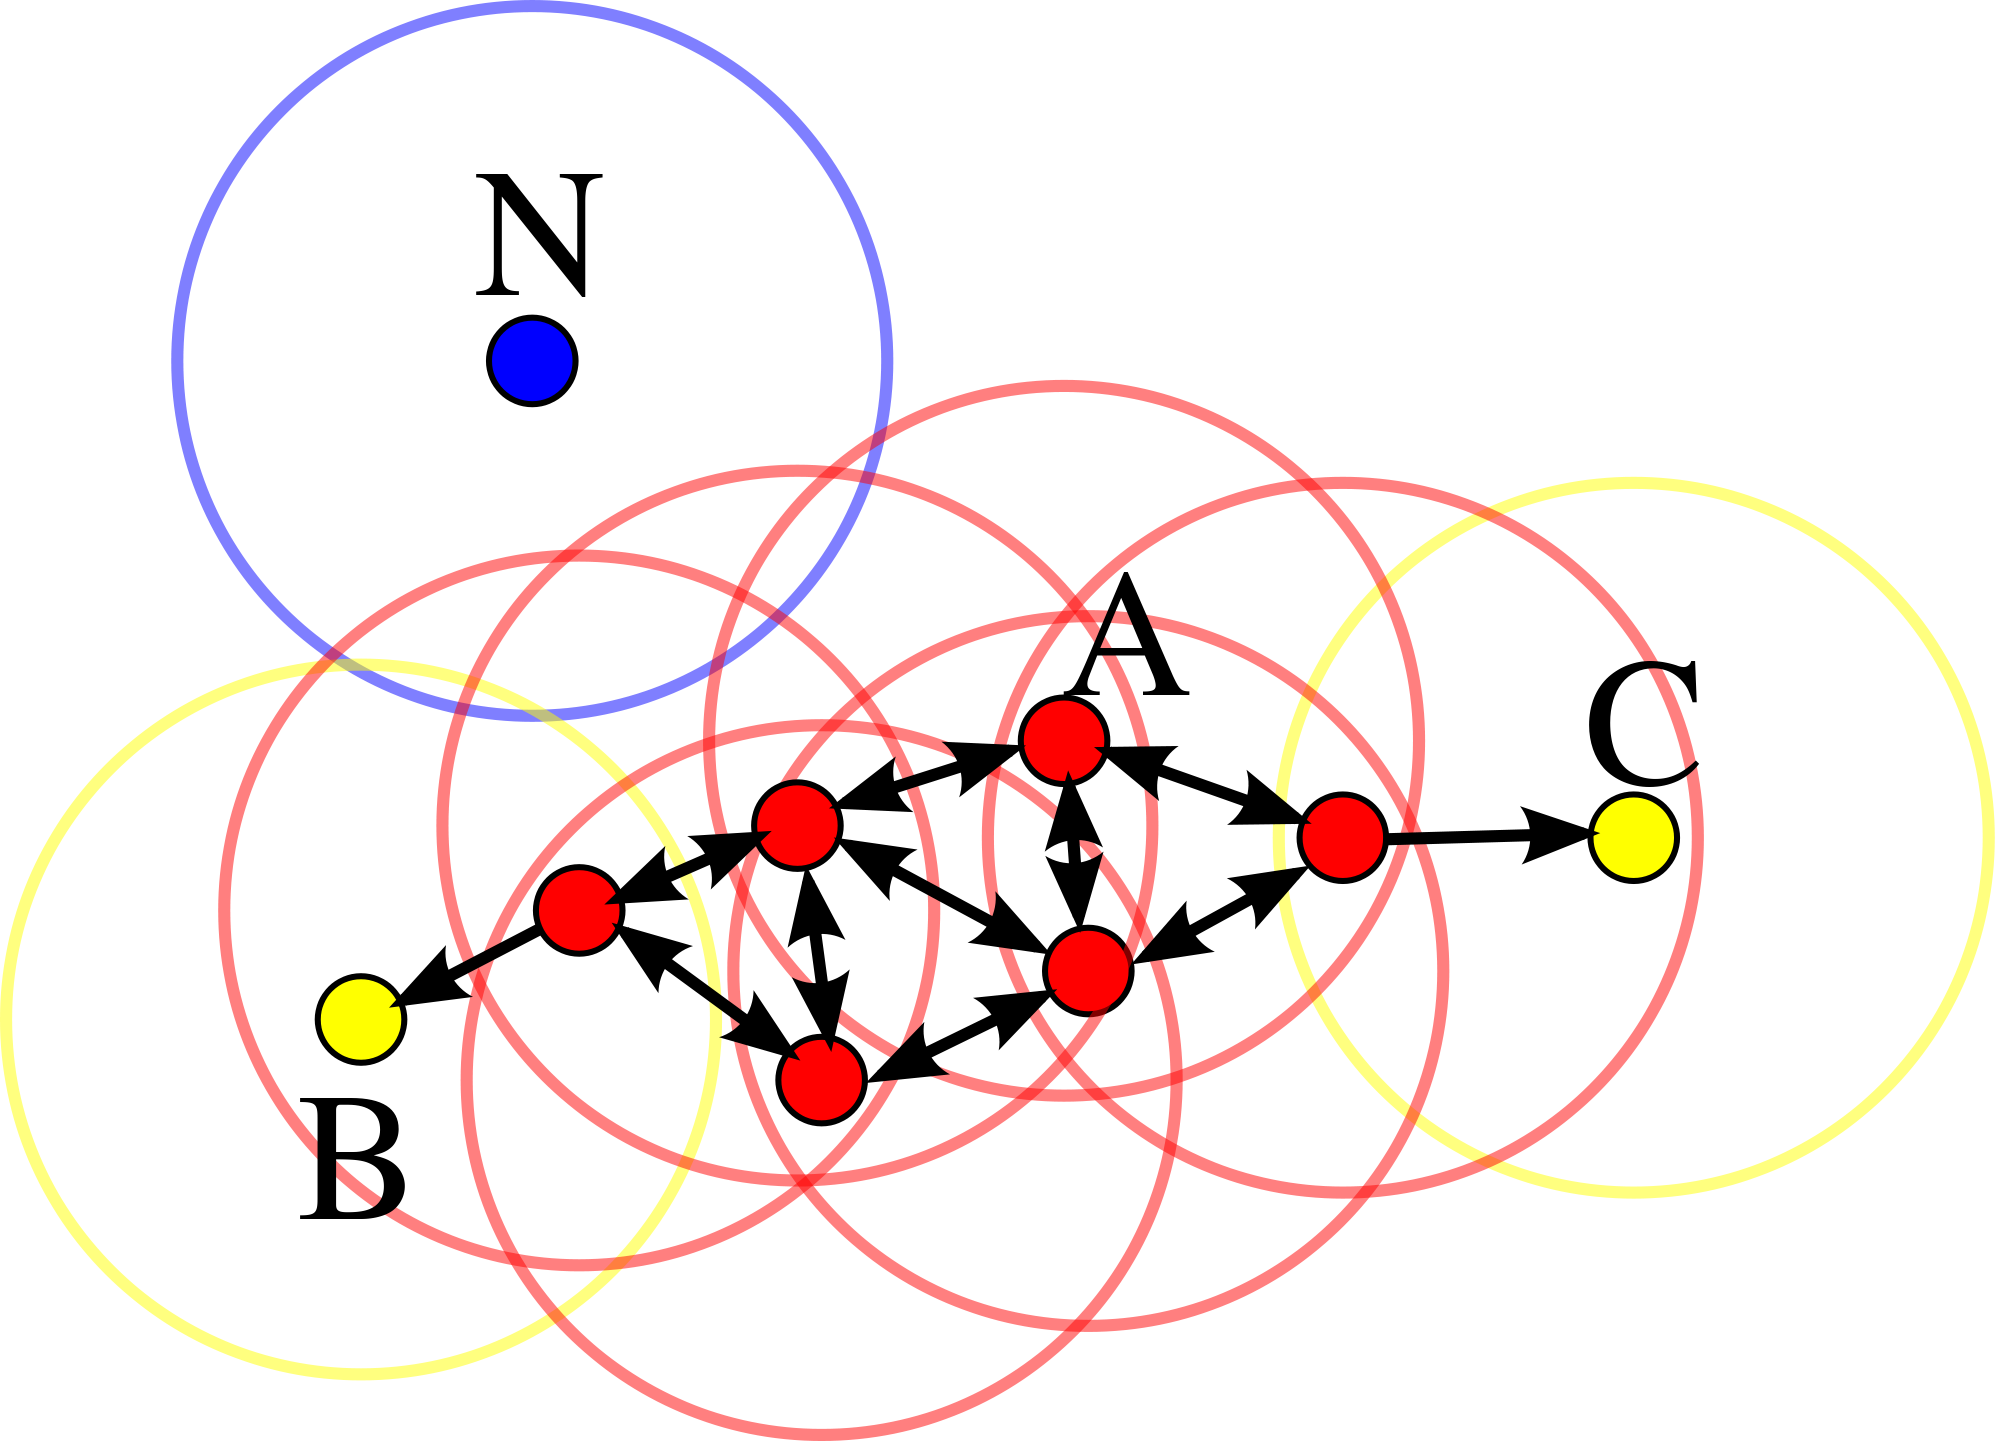
\includegraphics[width=0.6\textwidth]{2000px-DBSCAN-Illustration.png}
	\end{center}
	\caption{DBScan clustering algorithm illustration. Starting from a point within cluster A, and terminating at B and C, which do not contain enough points within their radius to be considered densely connected. N is never touched by this iteration of the algorithm as regions A, B and C are outside distance $\epsilon$.}
	\label{fig:dbscan}

\end{figure}

\begin{algorithm}[tb]
	\SetAlgoLined
	\KwData{$N \times N$ matrix: $D$}
	\KwResult{List of densely related points} 
	\bigskip
	DBScan($D$, $\epsilon$, MinPts): \\
	\ForEach {unvisited point $P$ in dataset $D$}
	{
		mark $P$ as visited; \\
		NeighbourPts $\leftarrow$ regionQuery($P$, $\epsilon$); \\
		\If{count of NeighbourPts $< \gamma$}{
			mark $P$ as noise; \\
		} 
		\Else {
			$C \leftarrow$ next cluster \\
			expandCluster($P$, NeighborPts, $C$, $\epsilon$, MinPts);
		}
	}
	\bigskip
	expandCluster($P$, NeighborPts, $C$, $\epsilon$, MinPts):  \\
	add $P$ to cluster $C$ \\
	\ForEach {point $P'$ in not visited}{
		mark $P'$ as visited; \\
		NeighbourPts' $\leftarrow$ regionQuery($P'$, $\epsilon$); \\
		\If{count of NeighbourPts' $>=$ MinPts} {
			NeighbourPts $\leftarrow$ NeighbourPts joined with NeighbourPts'; \\
		}
		\If{$P'$ is not yet a member of any cluster} {
			add $P'$ to cluster $C$'
		}
	}
	\bigskip
	regionQuery($P$, $\epsilon$):  \\
	{
 		return all points within $P'$ $\epsilon$-neighbourhood (including $P$)
	}
	\bigskip
	\caption{DBScan pseudo code}
	\label{alg:dbscan}
\end{algorithm}

Four parameters are required to uniquely characterize planes, in this case we use the Hessian plane form with parameters $(N_A, N_B, N_C, D)$. Hence our DBScan implementation operates in this four dimensional space, with the normal components coming from the normal estimator and the $D$ components mathematically derived from xyz and N spaces. An example of the clustering is shown in Figure~\ref{fig:box_normal_clustering}.

\subsection{DBScan Optimisations} % (fold)
\label{sub:dbscan_optimisations}

% subsection dbscan_optimisations (end)

Modifications to the DBScan algorithm were made to decrease the running time. By using tag fields to set whether points had already been visited or were already part of a cluster (a point can belong to one cluster only), the region query was prevented from being performed on points already part of a cluster. Further a custom conditional insertion procedure to insert into a list-like data structure without duplication was created, decreasing the complexity of insertion from $O(m \cdot log(n))$ (if using the standard template library set object) to $O(m)$.

The DBScan algorithm completes in $O(n^2)$ if the region query completes in $O(n)$, and $O(n \cdot log(n))$ if the region query completes within $O(log(n))$. Our implementation lay somewhere between the two, having a complexity dependent on run time, where a field of view containing more planar features took closer to the upper boundary. This is because captures with large or many planar features cause the region query procedure to be invoked more often, shifting the runtime complexity towards $O(n^2)$.

To combat against the possibility of slow run-time performance, it was decided to use a 2 step algorithm. A simple Flood Fill algorithm fills the initial field of view captured from the depth camera by flooding (clustering) connected points which have the same plane equation (remember the xyz-Normal point cloud is converted to a plane cloud once the vision module receives a frame from the RGB-D camera). The Flood Fill will generate a new set of planes, typically of a plane count less than 10. This will then be passed to the DBScan algorithm for the second step of the two step algorithm. Where as the Flood Fill algorithm moved only between neighbouring points, the DBScan looks over the whole image space to find points within tolerance $\epsilon$ of the seed point plane equation. Planes which are partially obscured or divided  will still be recognised as a single plane in DBScan. This is not the case in Flood Fill, and hence why a 2 step algorithm is employed. The Flood Fill rapidly finds planes and the slower DBScan corrects for any planes that have been segmented. Using the analogy of a graphical editing package, if the Flood Fill is the paint bucket tool, the DBScan is the patching tool.

\begin{algorithm}[tbp]
	\SetAlgoLined
	\KwData{$N \times N$ matrix: $D$}
	\KwResult{List of sets of connected points} 
	\bigskip
	FloodFill($P_{seed}$, MinPts): \\
	Push $P_{seed} \rightarrow$ Q \\
	\While {Q is not empty}
	{
	 	Pop $Q \rightarrow P$ \\
		\If{$P$ plane components within $\epsilon$ tolerance of $P_{seed}$}{
		Add $P$ to set $S$ \\

		\If{$P$ not in $Q$} {
			Push $P \rightarrow Q$ \\
			\ForEach{$H$ as direction (West, East, North, South)}{

				\If{$H$ not in $Q$}{
					Push $H \rightarrow Q$
				}

			}
		}


		}
	}
	\bigskip
	\caption{Flood Fill pseudo code for a single fill area}
	\label{alg:flood_fill}
\end{algorithm}

This design leads to increased throughput as the Flood Fill deals with the raw data from CCD space, converting 19200 points to only a few planes. The DBScan, having complexity towards a greedy $O(n^{2})$, only works on the plane set generated by the Flood Fill algorithm, meaning the near-quadratic complexity does not dominate run time as there are much less planes than there are points.

\subsection{The Flood Fill Algorithm}
\label{sub:flood_fill_algo}
As mentioned, the Flood Fill algorithm is analogous to a paint bucket function in a graphical editing package. The algorithm begins by randomly selecting a seed plane from the plane cloud (that is we randomly select a point and corresponding normal from the RGB-D camera sensor output), and proceed to fill out from this seed in all directions until the planes parameters $(N_A, N_B, N_C, D)$ differ by more than a value $\epsilon$ from the original seed plane. This forms a connected region, which represents a plane. Algorithm~\ref{alg:flood_fill} lists how given a seed point, a region fill is generated.

Once a single fill has terminated and more than a certain threshold of the image has either been filled (call it $\sigma$, i.e. 90\%) then the algorithm terminates. If this threshold has not been satisfied then begin a new fill, selecting a new random seed point from a point that has not been already included in a previous fill region. The algorithm will repeat until $\sigma$ is satisfied or it has attempted to flood fill the plane cloud for more than a certain number of times (call it $\gamma$, i.e. 50). The Flood Fill algorithm works iteratively using only a simple queue structure and list keep track if points have been explored yet in the context of the current fill or already added to a previous fill (plane) respectively, resulting in a linear complexity of $O(n)$. 


\subsection{Complications and Caveats in Segmentation} % (fold)
\label{sub:complications_in_the_segmentation_algorithm}

% subsection complications_in_the_segmentation_algorithm (end)

Complications arose when performing the flooding. As explained before, the projected grid from the RGB-D camera opens in a conic fashion. This means that objects closer the RGB-D camera will be showered in points, while those further away will contain far fewer points. This drop off happens at a quadratic rate, meaning the error in distance also occurs at a quadratic rate. To deal with this, the condition on the D parameter for which a point to be considered within the region was modified. As depth increases we open the parameter quadratically by projecting the z component of the plane normal onto the quadratic point z component. We do this for both the seed point and the point being queried, taking their absolute values and sum. We then multiply this value by an adjusted epsilon value ($\epsilon_{depth}$). 


The conditions (which all must be satisfied) for accepting a point into the current fill region becomes:
\begin{align}
|P_{seed|A} - P_{A}| &< \epsilon \\
|P_{seed|B} - P_{B}| &< \epsilon\\
|P_{seed|C} - P_{C}| &< \epsilon\\
|P_{seed|D}-P_{D}| &< (|N_{seed|z} \times P^{2}_{seed|z}| + |N_{z} \times P^{2}_{z}|) \times \epsilon_{depth}
\end{align}
where as before the last equation was the same as the previous three, except changed to the D parameter.
Note that P is the point which is under test (to investigate whether it should exist in the flood region), while $P_{seed}$ is the seed point at which was first chosen to characterise the Flood Fill region. 

Unforeseen consequences arose from the Flood Fill algorithm where the algorithm randomly selects a seed point near a vertex. The problem is that in order to get realistic normal components, the integral image normal estimation performs an averaging operation over normals in a kernel space of 40x40 normals. This means that high frequency information is lost, as shown in Figure~\ref{fig:spurious_plane_normals}. Hence, when the flood fill algorithm is filling out, spurious long thin planes may be generated along edges, giving rise to a false positive. 

In an effort to deal with this caveat, introducing an additional step between the Flood Fill and the DBScan which detects for false positives was undertaken. By computing the covariance matrix in xyz space for each point in a cluster, then finding the eigenvalues of this matrix calculates the PCA of each plane allowing us the investigate the dimensionality of each plane by checking the ratio of Eigen values generated. If there is much disparity, it can be assumed that a plane has been encountered fitting to the caveat described above and hence the plane is removed from the set of planes generated by the Flood Fill algorithm. 

The PCA was never implemented as it was found that by increasing the minimum number of points required for a fill region to be classified as a plane fixed the issue sufficiently for the purpose of this project. Additionally, it was decided to remove the DBScan algorithm altogether as it was realised that although planes occasionally become segmented using the Flood Fill, in practice running DBScan after Flood Fill made no measurable performance difference to the Kalman filter.




% \begin{figure}[p]
% 	\centering
% 	\subfloat[ in normal space. A total of 4 planes were found:, the floor, the white boards and two back walls] 
% 	{
% 		\label{fig:dbscan_planes}
% 		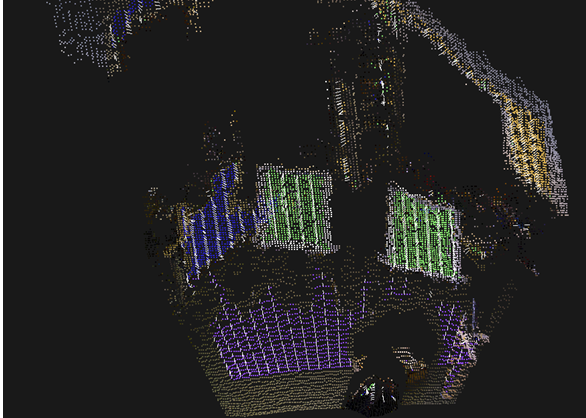
\includegraphics[width=0.4\textwidth]{6normal_boards.png}
% 	}
% 	\;
% 	\subfloat[of a laboratory in xyz space. Each white board is considered a separate cluster. Distant objects coloured in blue.] {
% 		\label{fig:table_dbscan}
% 		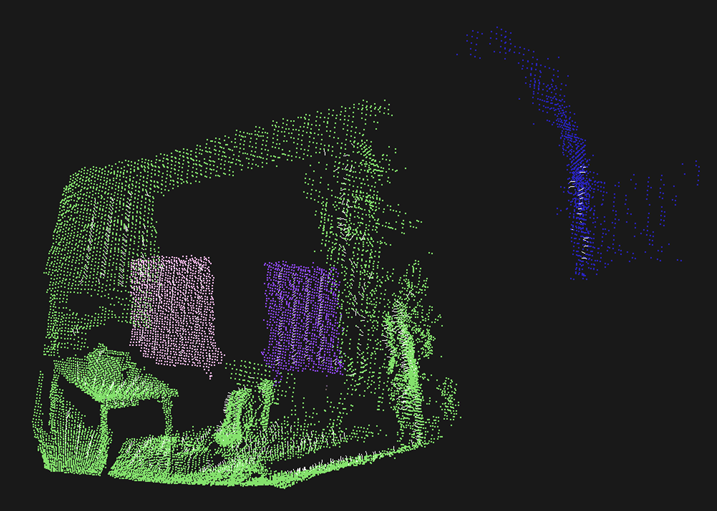
\includegraphics[width=0.4\textwidth]{6table_dbscan.png}

% 	}
% 	\caption{Images}
% 	\label{fig:DBSCAN_LAB}

% \end{figure}

\begin{figure}[p]
	\centering     %%% not \center
	\subfloat[Box before applying DBScan algorithm in normal space]{
		\label{fig:6box_before}
		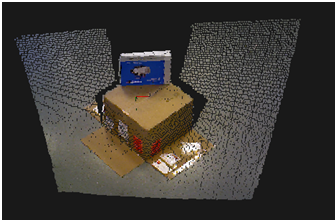
\includegraphics[width=0.4\textwidth]{6box_before.PNG}
	}
	\;
	\subfloat[Box after applying DBScan algorithm in normal space]{
		\label{fig:6box_after}
		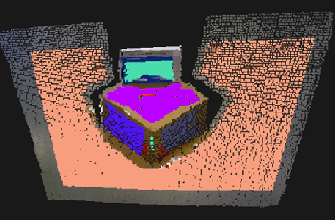
\includegraphics[width=0.4\textwidth]{6box_after.PNG}
	}

	\caption{Cluster using DBScan in normal space}
	\label{fig:box_normal_clustering}
\end{figure}




\clearpage

% section feature_extraction (end)

\clearpage %todo temp!
\section{Extended Kalman Filter} % (fold)
\label{sec:ekf}

To estimate the state of the system we employ the EKF which is the non-linear version of the regular Kalman Filter: the optimal state estimation filter for linear systems \cite{todo} with Gaussian noise.
When supplied with an accurate system model, and its statistical properties, the Kalman Filter provides the state estimate with the minimum mean-squared error \cite{todo}.
The extended version of the filter provides a near-optimal estimate of the system's state by linearising it around the current state estimate.
The reason why we need the non-linear version of the filter is due to the fact that the model includes rotations, which are non-linear in nature.
Furthermore, as our system has very many sources of noise for each modelled noise variable, we can assume from the central limit theorem that the noise is approximately Gaussian.
In practice, the assumption of approximately Gaussian noise works well in practice, and is used in many navigation applications \cite{todo}.

% We use a kalman filter... the optimal state estimator
% non linear due to rotations -- ekf
% 	euler vs runge kutta integrator
% 		very complicated linearization equations
% 			can be overcome with unscented kalman
% 		euler is fine if sampling fast enough
% 			if deltaT is small

Our system model can be described as a six DoF rigid body with Newtonian mechanics.
We do not model the aerodynamics of the craft and thus must rely on inertial sensors that gives information on the evolution of the system, similar to  \cite{OpenPilotPaper}.
The alternative would be to model the aerodynamics of the craft and the forces acting on the it. Our approach allows us to apply our model to any craft.
Complex phenomena such as the turbulence caused by the thrust channelled around in the confined space would be close to impossible to model.
Thus, our approach has the advantage that modelling-errors are minimised, and the time required for system identification is reduced.

\subsection{Filter Equations} % (fold)
\label{sub:filter_equations}
The notation of this section uses lower case letters for vectors and functions, and upper case letters for matrices. 

The Extended Kalman Filter is based on the following discrete time state space update model
\begin{align}
	x_k &= f(x_{k-1}, u_{k-1}, w_{k-1}) \notag \\
	y_k &= h(x_k, v_k)
	\label{eqn:system}
\end{align}
where $x_k$ is the state vector at time $k$, $f$ is the state transition function, $u$ is the control input vector at time $k$, $w_k$ is the process noise vector at time $k$, $y_k$ is the measurement vector at time $k$, $h$ is the function that maps the state space to the observed space, and $v_k$ is the measurement noise vector.

The EKF assumes the noise in the system to be Gaussian white noise as follows
\begin{align}
	w_k &\sim N(0,Q_k) \notag \\
	v_k &\sim N(0,R_k) \notag \\
	x_0 &\sim N(\hat{x}_0,P_0)
	\label{eqn:noisedef}
\end{align}
where $Q_k$ and $R_k$ are the process noise and measurement noise covariance matrices, at time $k$, respectively. The initial state estimate error is assumed to be drawn from a normal distribution with covariance $P_0$.

We define the notation
\begin{align}
	\hat{x}_{k|i} 	&= \mathbb{E}[x_k|y_0 \hdots y_i] \\
	P_{k|i} 		&= \operatorname{cov}(x_k - \hat{x}_{k|i}) \notag \\
					&= \mathbb{E}[ (x_k-\hat{x}_{k|i}) (x_k-\hat{x}_{k|i})^\top | y_0 \hdots y_i]
\end{align}
where $\hat{x}_{k|i}$ is the state estimate at time $k$ given observations of the system output up to and including time $i$, and $P_{k|i}$ is the covariance matrix associated with the error of the state estimate at time $k$ given given observations of the system output up to and including time $i$.

Given the above definitions and assumptions, we can predict the evolution of the system as follows
\begin{align}
	\hat{x}_{k|k-1} &= f(\hat{x}_{k-1|k-1}, u_{k-1}, \mathbb{E}[w_{k-1}])
	\label{eqn:predictx}
\end{align}
where we assume that the noise has zero mean:
\begin{align}
	\mathbb{E}[w_{k-1}] &= 0
\end{align}

The EKF uses a linearised version of the system model $f$, represented as a Jacobian matrix $F$. We use this matrix to transform the state error covariance matrix at each time step. We also account for the process noise $w$ using the Jacobian matrix $G$. This is computed as follows:
\begin{align}
	P_{k|k-1} &\approx F_{k-1} P_{k-1|k-1} F_{k-1}^\top + G_{k-1} Q_{k-1} G_{k-1}^\top
	\label{eqn:predictP}
\end{align}
where
\begin{align}
	F_{k-1} &= \left . \frac{\partial f}{\partial x} \right \vert _{\hat{x}_{k-1|k-1},u_{k-1}} \\
	G_{k-1} &= \left . \frac{\partial f}{\partial w} \right \vert _{\hat{x}_{k-1|k-1},u_{k-1}}
\end{align}

In order to correct for errors in the state estimate that has been accumulated due to the process noise, we incorporate corrections based on measurements made from the output of the system. To do this, we use the EKF update equations, which are described below.

For each measurement, such as a observed plane equation or a sonar altitude reading, we compute the expected measurement given our current state estimate. This is done using $h$, the measurement model, which maps the state space to the observed space.
This will be two distinct functions for sonar and plane measurement.
We compute the difference between this expected measurement, and the actual measurement, which we define as $z_k$. We also use the covariance associated with the measurment error $R$ to compute the covariance matrix associated with $z_k$ using a linear approximation of the measurement model $h$ denoted as $H$. This update equations are presented below:
\begin{align}
	\label{eqn:measurement_model}
	z_k &= y_k - h(\hat{x}_{k|k-1}, \mathbb{E}[v_k]) \\
	S_k &= \operatorname{cov}(z_k) \notag \\
		&\approx H_k P_{k|k-1} H_k^\top + R_k
\end{align}
where $P$ and $R$ are defined in equation (\ref{eqn:noisedef}), and where we assume that the noise has zero mean:
\begin{align}
	\mathbb{E}[v_k] &= 0
\end{align}
and where
\begin{align}
	H_{k} &= \left . \frac{\partial h}{\partial x} \right \vert _{\hat{x}_{k|k-1}}
	%V_{k} &= \left . \frac{\partial h}{\partial v} \right \vert _{\hat{x}_{k|k-1}}
\end{align}

We compute the updated state estimate, and the corresponding updated state estimate covariance matrix, as follows:
\begin{align}
	\hat{x}_{k|k} 	&= \hat{x}_{k|k-1} + K_k z_k \\
	P_{k|k} 		&\approx (I - K_k H_k) P_{k|k-1}
\end{align}
where the optimal Kalman gain $K$ is defined as follows:
\begin{align}
	K_k &= P_{k|k-1} H_k^\top S_k^{-1}
\end{align}
which is the gain that yields the MMSE estimates when used \cite{BerkelyCourse}.

% subsubsection filter_equations (end)

\subsection{System Model} % (fold)
\label{sub:system_model}

\begin{figure}[tb]
	\begin{center}
		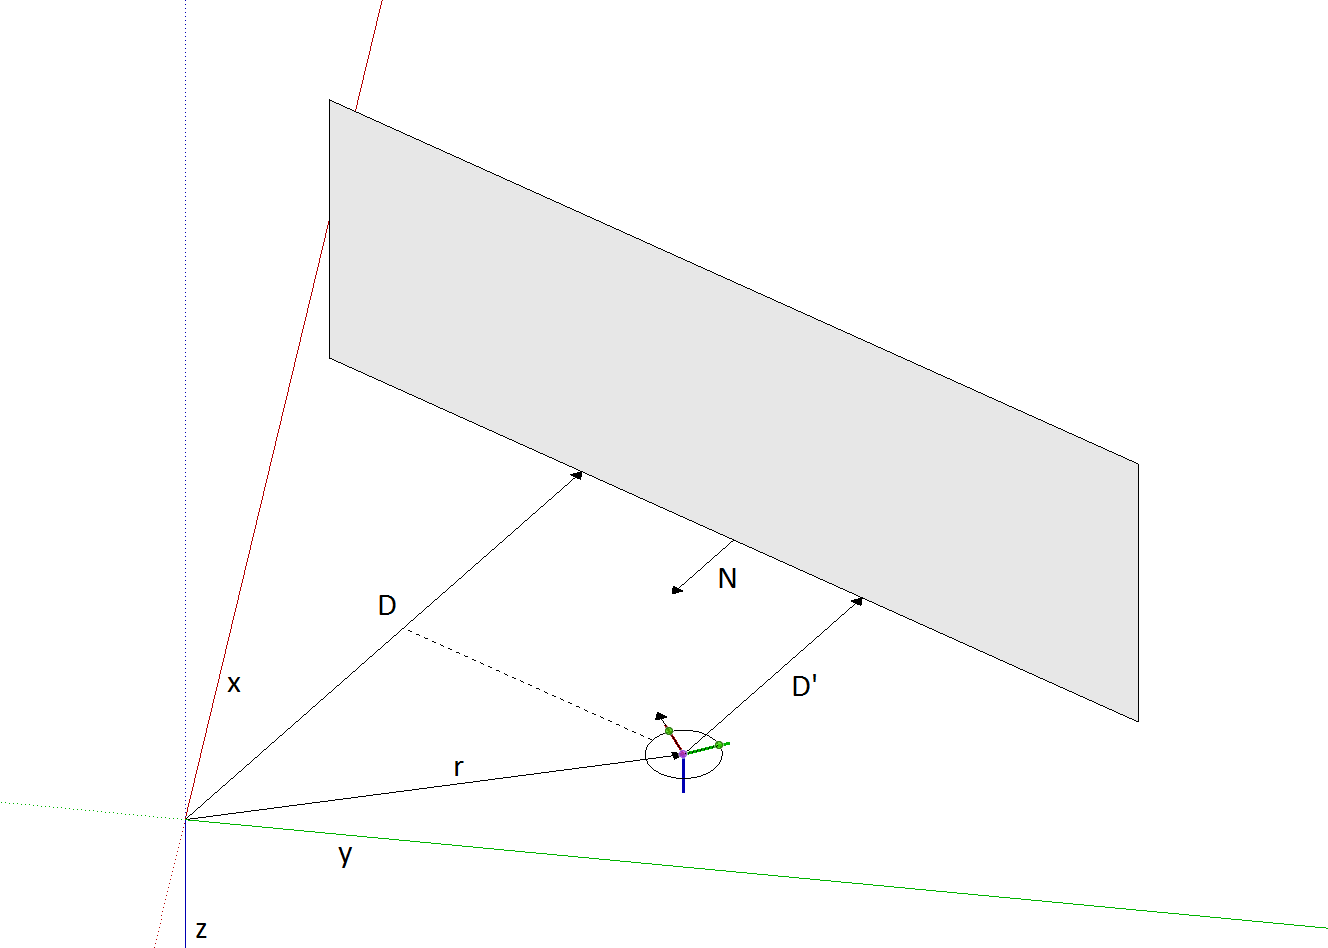
\includegraphics[width=0.8\textwidth]{coordinatesystem.png}
	\end{center}
	\caption{Coordinate system and plane equation representations. The craft is depicted as a circle in the bottom centre of the diagram. The position of the craft is represented using the position vector $r$ in the world coordinate system, and the local coordinate axes in the body frame are depicted on the craft.
	A plane is represented by its normal vector, $N$ and its distance from the origin, $D$, in the world coordinate system. When observed by the craft, the plane is seen as the normal vector in the body coordinate system and the distance $D'$. It is clear from the figure that the difference between $D$ and $D'$ is the projection of $r$ along $N$.} \label{fig:coordinatesystem} \end{figure}

In order to evaluate the equations from the previous section, we need to establish a model of the system. The state vector is segmented into two parts, the robot state and the map state. Each consists of several components, as listed below:
\begin{align}
	\label{eqn:state}
	x &=
	\left[
	\begin{matrix}
		x_r \\
		x_m
	\end{matrix}
	\right]
	=
	\left[
	\begin{matrix}
		r \\
		v \\
		q \\
		b_\omega \\
		b_a \\
		\\
		\pi_0 \\
		\vdots \\
		\pi_{n-1}
	\end{matrix}
	\right]
	&
	\dot{x} &= 
	\left[
	\begin{matrix}
		\dot{r} \\
		\dot{v} \\
		\dot{q} \\
		\dot{b}_\omega \\
		\dot{b}_a \\
		\\
		\dot{\pi}_0 \\
		\vdots \\
		\dot{\pi}_{n-1}
	\end{matrix}
	\right]
\end{align}

where $x_r$ represents the state of the craft, $x_m$ represents the state of the feature map, $r$ is the position of the craft in the inertial frame, $v$ is the velocity in the inertial frame, $q$ is the quaternion that represents the attitude of the craft: a rotation from the inertial frame to the body frame, $b_\omega$ and $b_a$ represent the gyro and accelerometer bias, respectively. $\pi_0 \hdots \pi_{n-1}$ are the equations of the planes currently stored in the map. The axes conventions are: $x$ points along North, $y$ along East, and $z$ points down. Angular rates are defined as right hand rotations along each of these axes, and the following quaternion convention:
\begin{align}
	\label{eqn:quaternion_components}
	q = q_0 + q_1i + q_2j + q_3k
\end{align}

We segment the $P$ matrix into blocks consisting of sub-matrices to do with either the robot or to do with the map, or to do with the cross-covariance of the two. We can extend this subdivision so that it considers each plane separately, as suggested by \cite{Sola2013}.
This will be useful when computing Equation~(\ref{eqn:H}).
\begin{align}
	P &=
	\left[
	\begin{matrix}
		P_{rr} 	& P_{rm} \\
		P_{mr} 	& P_{mm}
	\end{matrix}
	\right]
	=
	\left[
	\begin{matrix}
		P_{rr} 		& P_{r \pi_1} 		& \cdots 	& P_{r \pi_n} \\
		P_{\pi_1 r} & P_{\pi_1 \pi_1}	& \cdots 	& P_{\pi_1 \pi_n} \\
		\vdots		& \vdots 			& \ddots 	& \vdots \\
		P_{\pi_n r} & P_{\pi_n \pi_1} 	& \cdots 	& P_{\pi_n \pi_n}
	\end{matrix}
	\right]
	\label{eqn:Pparts}
\end{align}

The state vector as defined in Equation~(\ref{eqn:state}) consists of the following components:
\begin{align}
	r &= 
	\left[
	\begin{matrix}
		x \\
		y \\
		z
	\end{matrix}
	\right]
	&
	v &=
	\left[
	\begin{matrix}
		\dot{x} \\
		\dot{y} \\
		\dot{z}
	\end{matrix}
	\right]
	&
	q &=
	\left[
	\begin{matrix}
		q_0 \\
		q_1 \\
		q_2 \\
		q_3
	\end{matrix}
	\right]
	&
	b_\omega &=
	\left[
	\begin{matrix}
		b_{\omega_x} \\
		b_{\omega_y} \\
		b_{\omega_z} 
	\end{matrix}
	\right]
	&
	b_a &=
	\left[
	\begin{matrix}
		b_{a_x} \\
		b_{a_y} \\
		b_{a_z} 
	\end{matrix}
	\right]
	&
	\pi &=
	\left[
	\begin{matrix}
		N_x \\
		N_y \\
		N_z \\
		D
	\end{matrix}
	\right]
\end{align}

The derivative of the state vector is computed in order to propagate the state over time.
\begin{align}
	\label{eqn:xdotDef}
	\dot{r} &= v
	&
	\dot{v} &= R_{eb}(q) a
	&
	\dot{q} &= \frac{1}{2}\Xi(q) \omega
	&
	\dot{b}_\omega &= w_{b\omega}
	&
	\dot{b}_a &= w_{ba}
	&
	\dot{\pi} &= 0
\end{align}

where $a$ and $\omega$ are the true body frame accelerations and angular rates, respectively.
$R_{eb}$ is the body to earth rotation matrix and $\Xi$ is the matrix that maps the body frame angular rates to the rate of change of quaternion. Both of these matrices are a function of the current craft orientation, that is, a function of $q$, and are defined below in Equations~(\ref{eqn:Xi}) and (\ref{eqn:Omega}).

The system model $f$, described in Equation~(\ref{eqn:system}) and (\ref{eqn:predictx}), operates in discrete time, but we have established our model in continuous time. As such, we perform a first order approximation to the continuous time system:
\begin{align}
	f &= x + \Delta T \dot{x}
	\label{eqn:descrete_f}
\end{align}

Defining the model further, we have that
\begin{align}
	\omega &= \omega_m + w_\omega - b_\omega &
	a &= a_m + w_a - b_a + g_b
\end{align}
where $a_m$ and $\omega_m$ are the measured accelerations and angular velocities in the body frame, respectively, and $g_b$ is the acceleration due to gravity in the body frame.

Defined in Equation~(\ref{eqn:proc_noise_def}) is the process noise vector. The first two components are comprised of the additive noise in the measurement obtained from the gyro and accelerometer, respectively. This noise is modelled by simply measuring several minutes of output from the sensors and using the sample covariance matrix as the covariance that describes this additive noise.

The inertial sensors have an undefined zero-bias point. This means that the measurements have a bias that varies between chips, and over different temperatures and supply voltages. This semi-random variation of the bias point is modelled as a random walk. That is, we model this variation as a bias state that is perturbed by an additive noise term.
To measure this term, we computed the discrete time derivative of the output of the sensor during the same stationary test, and low-pass filtered the result. The time constant of the low pass filter, 5 seconds, was selected heuristically to represent a probable timebase over which temperature variations would start to play a significant role. The sample covariance matrix of the resultant metric is used to characterise the bias drift random variable.
\begin{align}
	\label{eqn:proc_noise_def}
	w &= 
	\left[
	\begin{matrix}
		w_\omega \\
		w_a \\
		w_{b\omega} \\
		w_{ba}
	\end{matrix}
	\right]
	% \omega_w0 = 
	% \begin{bmatrix}
	% 	 0.0001679  &-6.15e-05 &-0.0001051 \\
	% 	 -6.15e-05   &0.000132 & -6.54e-05\\
	% 	-0.0001051  &-6.54e-05 & 0.0002536\\
	% \end{bmatrix}
	% \right]
	% \omega_a0 = 
	% \begin{bmatrix}
	% 	 0.000667   3.77e-05  -6.48e-05 \\
	% 	 -3.77e-05  0.0008222 -0.0001422\\
	% 	--6.48e-05 -0.0001422  0.0027314\\
	% \end{bmatrix}
	% \right]
	% \omega_bw0 = 
	% \begin{bmatrix}
	% 	 0.0003552  -3.23e-05 -0.0002509 \\
	% 	 3.23e-05  0.0002822 -0.0002381\\
	% 	-0.0002509 -0.0002381  0.0005686\\
	% \end{bmatrix}
	% \right]
	% \omega_ba0 = 
	% \begin{bmatrix}
	% 	 0.003501  -0.001312   0.002149 \\
	% 	 -0.001312   0.004719  -0.002273\\
	% 	 0.002149  -0.002273    0.01367\\
	% \end{bmatrix}
	% \right]
\end{align}

The derivation of the rate of change of the quaternion with respect to angular velocity in the body frame, shown in Equations~(\ref{eqn:Xi}) through (\ref{eqn:lastQuatInt}) can be found in \cite{MARSlab} (see equation 108)
Note that they use the convention $q = q_4 + q_1i + q_2j + q_3k$, while we use the convention shown in Equation~(\ref{eqn:quaternion_components}), which is the same convention used by MATLAB's Aerospace Blockset \cite{MATLABAerospace}, and the OpenPilot implementation \cite{OpenPilotPaper}.


\begin{align}
	\label{eqn:Xi}
	\Xi(q) &=
	\left[
	\begin{matrix}
		-q_1 	& -q_2	& -q_3 	\\
		q_0		& -q_3 	& q_2 	\\
		q_3 	& q_0 	& -q_1 	\\
		-q_2 	& q_1 	& q_0
	\end{matrix}
	\right]
\end{align}

\begin{align}
	\label{eqn:Omega}
	\Omega(\omega) &=
	\left[
	\begin{matrix}
		0 			& -\omega_x 	& -\omega_y	& -\omega_z	\\
		\omega_x 	& 0 			& \omega_z 	& -\omega_y \\
		\omega_y 	& -\omega_z 	& 0 		& \omega_x 	\\
		\omega_z 	& \omega_y		& -\omega_x & 0
	\end{matrix}
	\right]
\end{align}

\begin{align}
	\dot{q} 	&= \frac{1}{2} \Omega(\omega) q \\
	\label{eqn:lastQuatInt}
				&= \frac{1}{2} \Xi(q) \omega
\end{align}

The derivation of the quaternion derived rotation matrix is also shown in \cite{MARSlab} (see equation 91) and is defined as follows
\begin{align}
	R_{be}(q) &=
	\left[
	\begin{matrix}
		2(q_0^2 + q_1^2) - 1 	& 2(q_1 q_2 + q_0 q_3) 	& 2(q_1 q_3 - q_0 q_2) \\
		2(q_1 q_2 - q_0 q_3) 	& 2(q_0^2 + q_2^2) - 1 	& 2(q_2 q_3 + q_0 q_1) \\
		2(q_1 q_3 + q_0 q_2)	& 2(q_2 q_3 - q_0 q_1)	& 2(q_0^2 + q_3^2) - 1
	\end{matrix}
	\right]
\end{align}

Furthermore, as a rotation matrix is orthogonal, we have that
\begin{align}
	R_{eb} &= R_{be}^\top
\end{align}

As the state transition model $f$ operates in discrete time, and more directly, because we have performed the discritisation shown in Equation~(\ref{eqn:descrete_f}), we derive the state transition Jacobian matrix, mentioned in Equation~(\ref{eqn:predictP}) as follows
\begin{align}
	F &= \frac{\partial f}{\partial x} \notag \\
	&=
	\label{eqn:descrete_F}
	I + \frac{\partial \dot{x}}{\partial x} \Delta T
	% &= 
	% I_{16+4n \times 16+4n} +
	% \left[
	% \begin{matrix}
	% 	0_{3\times3} 	& I_{3\times3} 	& 0_{3\times4} 	& 0_{3\times3} 		& 0_{3\times3} 	& 0_{3\times4n} \\
	% 	0_{3\times3}		& 0_{3\times3} 	& F_{vq}	& 0_{3\times3} 		& F_{vb_a} 	& 0_{3\times4n} \\
	% 	0_{4\times3}		& 0_{4\times3} 	& F_{qq}	& F_{qb_\omega}	& 0_{4\times3}	& 0_{4\times4n} \\
	% 	0_{3\times3}		& 0_{3\times3}	& 0_{3\times4} 	& 0_{3\times3} 		& 0_{3\times3} 	& 0_{3\times4n} \\
	% 	0_{3\times3}		& 0_{3\times3}	& 0_{3\times4} 	& 0_{3\times3}		& 0_{3\times3}	& 0_{3\times4n} \\
	% 	0_{4n\times3} 		& 0_{4n\times3} 	& 0_{4n\times4} 	& 0_{4n\times3}		& 0_{4n3\times3} 	& 0_{4n\times4n}
	% \end{matrix}
	% \right] 
	% \Delta T
	% \\
\end{align}
Directly computing the Jacobian of the continuous time model from Equation~(\ref{eqn:xdotDef}), and assuming that the features of the map do not move, yields the following
\begin{align}
	F = I_{16+4n \times 16+4n} +
	%\left[
	%\begin{matrix}
	%	I_{16 \times 16} 	& 0_{16 \times 4n} \\
	%	0_{4n \times 16}	& I_{4n \times 4n}
	%\end{matrix}
	%\right]
	%+
	\left[
	\begin{matrix}
		\cdot 		& I_{3x3} 	& \cdot	 	& \cdot		 	& \cdot		& \cdot \\
		\cdot		& \cdot	 	& F_{vq}	& \cdot		 	& F_{vb_a} 	& \cdot \\
		\cdot		& \cdot	 	& F_{qq}	& F_{qb_\omega}	& \cdot		& \cdot \\
		\cdot		& \cdot		& \cdot	 	& \cdot		 	& \cdot		& \cdot \\
		\cdot		& \cdot		& \cdot	 	& \cdot			& \cdot		& \cdot \\
		\cdot		& \cdot		& \cdot	 	& \cdot			& \cdot		& \cdot
		%\dots 		& \vdots	& \vdots 	& \vdots		& \vdots	& \ddots
	\end{matrix}
	\right]
	\Delta T
	\label{eqn:F}
\end{align}
where
\begin{align}
	F_{vq} 	&= 2
	\left[
	\begin{matrix}
		F_{vq1} 	& -F_{vq0} 	& F_{vq3} 	& -F_{vq2} \\
		F_{vq2} 	& -F_{vq3} 	& -F_{vq0} 	& F_{vq1} \\
		F_{vq3} 	& F_{vq2} 	& -F_{vq1} 	& -F_{vq0}
	\end{matrix}
	\right]
%\end{align}
%where
%\begin{align}
	& F_{vq(0\cdots3)} &= \Xi(q) a
\end{align}
% that is
% \begin{align}
% 	%a &= a_m - b_a 							\notag 	\\
% 	F_{vq0} &= -q_1 a_x - q_2 a_y - q_3 a_z	\notag 	\\
% 	F_{vq1} &= q_0 a_x - q_3 a_y + q_2 a_z 	\notag	\\
% 	F_{vq2} &= q_3 a_x + q_0 a_y - q_1 a_z \notag	\\
% 	F_{vq3} &= -q_2 a_x + q_1 a_y + q_0 a_z
% \end{align}
%\begin{align}
%	&= 2
%	\left[
%	\begin{matrix}
%		q_0 a_x - q_3 a_y + q_2 a_z 	& q_1 a_x + q_2 a_y + q_3 a_z 	& -q_2 a_x + q_1 a_y + q_0 a_z 	& -q_3 a_x - q_0 a_y + q_1 a_z 	\\
%		q_3 a_x + q_0 a_y - q_1 a_z 	& q_2 a_x - q_1 a_y - q_0 a_z 	& q_1 a_x + q_2 a_y + q_3 a_z 	& q_0 a_x - q_3 a_y + q_2 a_z 	\\
%		-q_2 a_x + q_1 a_y + q_0 a_z 	& q_3 a_x + q_0 a_y - q_1 a_z 	& -q_0 a_x + q_3 a_y - q_2 a_z 	& q_1 a_x + q_2 a_y + q_3 a_z 	\\
%	\end{matrix}
%	\right]
%\end{align}
and
\begin{align}
	F_{vb_a} &= -R_{eb}(q)
%\end{align}
&
%\begin{align}
	F_{qq}	&= \frac{1}{2} \Omega(\omega)
			 %= \frac{1}{2} \Omega(\omega_m - b_\omega)
%\end{align}
&
%\begin{align}
	F_{qb_\omega} &= -\frac{1}{2} \Xi(q)
\end{align}

The process noise model is defined as follows
\begin{align}
	G &= \frac{\partial f}{\partial w} \notag \\
	&=
	\frac{\partial \dot{x}}{\partial w} \Delta T
\end{align}

By considering the way that the noise is modelled, and assuming that the process noise only affects the craft, we derive the following
\begin{align}
	G = \left[
	\begin{matrix}
		\cdot 			& \cdot 	& \cdot 		& \cdot \\
		\cdot 			& G_{vw_a} 	& \cdot 		& \cdot \\
		G_{qw_\omega}	& \cdot 	& \cdot 		& \cdot \\
		\cdot 			& \cdot 	& I_{3\times3}	& \cdot \\
		\cdot 			& \cdot 	& \cdot 		& I_{3\times3}
	\end{matrix}
	\right]
	\Delta T
\end{align}
where $\cdot$ represents null entries, and where
\begin{align}
	G_{vw_a} &= R_{eb}(q)
%\end{align}
&
%\begin{align}
	G_{qw_\omega} &= \frac{1}{2} \Xi(q)
%\end{align}
%&
%\begin{align}
%	G_{b_\omega w_{b\omega}} &= I_{3x3}
%&
%	G_{b_a w_{ba}} &= I_{3x3}
\end{align}

Having derived $F$ and $G$, we can use a sparse matrix optimisation that is based on the fact that the plane map features do not move. This technique, specific to EKF-SLAM, is developed in detail in \cite{Sola2013}.
This means that when calculating equation~(\ref{eqn:predictP}), we can use the sparsity of $F$ to simplify the calculation as follows:
\begin{align}
	F_r &= F_{(0-15,0-15)} \notag \\
	P &\leftarrow
	\left[
	\begin{matrix}
		F_r P_{rr} F_r^\top + GQG^\top 	& F_r P_{rm} \\
		P_{mr} F_r^\top 				& P_{mm}
	\end{matrix}
	\right]
\end{align}
where the parts of P are defined in equation~(\ref{eqn:Pparts}).

The forward observation model $h$ for the plane observation, as required by Equation~(\ref{eqn:measurement_model}), is derived below. Using this function we can compute the expected plane measurement given our current state estimate.
\begin{align}
	T_h &= 
	\left[
	\begin{matrix}
		R_{be} 	& 0_{3\times1} \\
		r^\top 	& 1
	\end{matrix}
	\right]
	\\
	h &= T_h \pi
\end{align}

We also need to define $H$, the Jacobian of $h$ w.r.t the state. The $H$ matrix is only a function of the robot's state and the particular plane observation in question and thus is composed of only two sections, one relating to the state, and one relating to the plane itself. As only the associated plane is relevant, only the part of the H matrix that pertains to this specific plane in the state is populated, and the other entries are set to zero.
In the implementation, we take advantage of this sparsity and compute matrix multiplication terms only related to the populated columns, as shown in \cite{Sola2013}.
For clairity, $H$ is built up using several submatricies as follows:
\begin{align}
	\tilde{q} &= 
	\left[
	\begin{matrix}
		-q_0 \\
		q_1 \\
		q_2 \\
		q_3
	\end{matrix}
	\right]
	&
	H_{Nq(0\cdots3)} &= \Xi(\tilde{q}) N_p
\end{align}
\begin{align}
	H_{Nq} &= 2
	\left[
	\begin{matrix}
		-H_{Nq1} 	& -H_{Nq0} 	& H_{Nq3} 	& -H_{Nq2} \\
		-H_{Nq2} 	& -H_{Nq3} 	& -H_{Nq0} 	& H_{Nq1} \\
		-H_{Nq3} 	& H_{Nq2} 	& -H_{Nq1} 	& -H_{Nq0}
	\end{matrix}
	\right]
\end{align}
\begin{align}
	\label{eqn:H}
	H &=
	\left[
	\begin{matrix}
		\begin{matrix}
			0_{3 \times 3} \\
			N_p^\top
		\end{matrix}
		& 0_{4 \times 3}
		&
		\begin{matrix}
			H_{Nq} \\
			0_{1 \times 4}
		\end{matrix}
		& 0_{4 \times 6}
		&
		%& 0
		& \cdots
		%& 0
		& T_h
		%& 0
		& \cdots
		%& 0
	\end{matrix}
	\right]
\end{align}
where $\cdots$ represents appropriately sized zero matricies.

Furthermore, we have a sonar sensor that measures the altitude of the craft with respect to the ground below it. For our purposes we assume that the floor is flat and has zero elevation. As such, we simply define it's measurement model as follows
\begin{align}
	h &= -z \notag \\
	H &= \left[
	\begin{matrix}
		0 & 0 & -1 & 0 & \cdots & 0
	\end{matrix}
	\right]
\end{align}

% subsection system_model (end)

\begin{figure}[tb]
	\begin{center}
		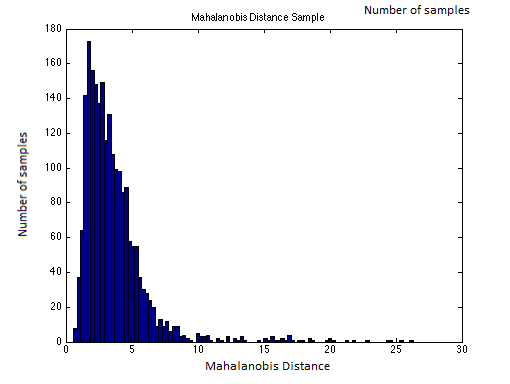
\includegraphics[height = 0.3\textwidth]{malhala_hist_100bins_10000datapoints_notmoving22}
	\end{center}
	\caption{Histogram showing the mahalanobis distance from the discovered planes to the reference planes in a stationary test with 10,000 data points.}
	\label{fig:mahaldisthist}
\end{figure}

\subsection{Landmark Association} % (fold)
\label{sub:landmark_association}
When a new plane measruement is generated by the depth camera and the vision system, we need to decide whether this plane exists in the map or not. To do this we use the statistical measure called the squared Mahalanobis distance to evaluate how closely a newly observed plane is related to the ones in the state map. This measure is best described as a normalised distance that is used to gauge similarity of a new sample to a distribution with a known covariance matrix. The measure is formally defined as

%\begin{aligned}
	%d = 
%\end{aligned}

We do 

When making the decision on whete

We use a threshold on this distance such that 99\% of true measurements are accepted. For our 4 dimensional plane measurement, this evaluates to:

\verb"d = chi2inv(0.99,4) = 13.2767" which is the MATLAB command for the inverse chi squared distribution with 4 degrees of freedom and evaluated at 0.99. In order to perform association, the procedure is we find the mahalanobis distance between our new observation and all the planes in the map, keeping the minimum. If this minimum is less than the threshold, then the data is associated, if not it is discarded as an outlier.

% subsection landmark_association (end)

\subsection{Landmark Initialization} % (fold)
\label{sub:landmark_initialization}
The ability to observe new planes as the craft explores its environment is crucial for it to keep track of its location. By re-observing these new features, the craft is able to compute corrections in its location. When the craft sees a new plane, it add this to its internal state transforming the plane equations in the body frame to the world frame and then storing this and its associated covariance information. It uses an inverse observation model, e which describes how we can derive the current state from an observed plane equation y. Mathematically we have,

\begin{align}
	y_{k} = y|_{x(k)} =  
	\left[
	\begin{matrix}
		\hat{N}_x \\
		\hat{N}_y \\
		\hat{N}_z \\
		\hat{D}
	\end{matrix}
	\right]
\end{align}

\begin{align}
	T_e &= 
	\left[
	\begin{matrix}
		R_{eb} 			& 0_{3\times1} \\
		-r^\top R_{eb}	& 1
	\end{matrix}
	\right]
\end{align}
$T_e$ defines the transformation matrix from the body frame to the earth frame. The new plane numbered j is defined below, 

\begin{align}
	\pi_j	&= e(y_k,x) \notag \\
			&= T_e y_k
\end{align}
The new state at time k now becomes, 
\begin{align}
	x_{k} &\leftarrow
	\left[
	\begin{matrix}
		x_{k} \\
		\pi_j
	\end{matrix}
	\right]
\end{align}
To update the P or state covariance matrix, we have to compute the jacobian of e w.r.t the state denoted as $E_x$ and the jacobiain w.r.t the newly observed plane denoted as $E_y$. Mathematically we have, 
\begin{align}
	E_y &= \frac{\partial e}{\partial y} \notag \\
		&= T_e \\
	E_x &= \frac{\partial e}{\partial x} \notag \\
		&=
	\left[
	\begin{matrix}
		\begin{matrix}
			0_{3 \times 3} \\
			-\hat{N}^\top R_{be}
		\end{matrix}
		&
		0_{4 \times 3}
		&
		\begin{matrix}
			E_{Nq} \\
			-r^\top E_{Nq}
		\end{matrix}
		&
		0_{4 \times 6}
	\end{matrix}
	\right]
\end{align}
where
\begin{align}
	E_{Nq} 	&= 2
	\left[
	\begin{matrix}
		E_{Nq1} 	& -E_{Nq0} 	& E_{Nq3} 	& -E_{Nq2} \\
		E_{Nq2} 	& -E_{Nq3} 	& -E_{Nq0} 	& E_{Nq1} \\
		E_{Nq3} 	& E_{Nq2} 	& -E_{Nq1} 	& -E_{Nq0}
	\end{matrix}
	\right]
\end{align}
where
\begin{align}
	E_{Nq(0\cdots3)} &= \Xi(q) \hat{N}
\end{align}
TODO(define Enq and N hat)
The updated P matrix is defined as: 
\begin{align}
	P_{\pi \pi} &= E_x P_{(0-15,0-15)} E_x^\top + E_y R E_y^\top \notag \\
	P_{x \pi} 	&= E_x P_{(0-15,all)} \notag \\
	P &\leftarrow
	\left[
	\begin{matrix}
		P 			& P_{x \pi}^\top \\
		P_{x \pi}	& P_{\pi \pi}
	\end{matrix}
	\right]
\end{align}

% subsection landmark_initialization (end)

\subsection{Optimisation} % (fold)
\label{sub:optimisation}

SerialUpdate: \cite{OpenPilotPaper} and chapter 4.2.2 of \cite{KFBookSerialupdate}, and also mentioned in \cite{Sola2013}
The referenced papers perform an optimization which assumes an entirely uncorrelated measurement noise covariance matrix. That is the $R$ matrix is purely diagonal.
We, on the other hand, use a measurement model that includes the measurement of planes. These measurements consist of the estimated plane equation in hessian normal form. As the plane is in a three dimensional space, and thus the measurement error will have three degrees of freedom, and this form has four dimensions, the covariance matrix cannot be uncorrelated.
That is, as the hessian normal form uses a unit vector, the length of this vector is bound to unity. As such, the probability distribution of the error of the components of this normal vector cannot be spherical.
In fact, after linearisation, this distribution is projected onto a plane tangential to the actual distribution. 
%TODO: insert picture of distrubution projected onto plane

While we cannot serialise the individual components of a plane measurement, the measurement error between planes are uncorrelated, so we can still make use of the serial update strategy. As such, at each time there is a new frame that has finished feature extraction, we serially apply the measurement updates for each plane, without running the predict loop in-between.
That means the update stage will only have to invert $v$ matrices of size $4\times4$, instead of inverting a $4v \times 4v$ matrix. 
As a further optimization, we find that the equation that transforms the state covariance matrix (\ref{eqn:predictP}) forms a separable system. That is, the Jacobian matrix $F$ as defined in (\ref{eqn:F}) does not carry any information regarding the craft to the planes, and vica versa.
In fact, all terms in $F$ regarding the planes are zero, except the main diagonal, which is unity. This means that not only is it a separable system, but the plane subsystem is fully static.
Because the system is separable, and because the second half is static, we can ignore the second half of the system when computing (\ref{eqn:predictP}).
This makes an enormous difference in the scalability of the Kalman filter approach. If the entire matrix-matrix multiplication is required, then the algorithm will scale like $O(n^3)$ where $n$ is the number of planes in the state vector. Now that this cubic dependence on $n$ is removed, only $O(n^2)$ terms remain, along with other terms.
%TODO: explore complexity
%TODO: incorporate reasoning from Sola2013

	We cross check our implementation against a similar open source implementation by the OpenPilot team %\cite{OpenPilotinsgps}. \cite{Holz2011}

% subsection implementation (end)

% section EKF (end)

\section{Testing and Results} % (fold)
\label{sub:testing_kalman}
In our test setup, we based our coordinate system in a vertex of the room as origin defining the x,y and z coordinates to be along the three wall edges connected to the origin vertex. Our test system consist of Mavrx's inertial measurement unit containing the inertial sensors and depth camera taped together. To ensure a functional kalman filter, full observability of system in the x,y and z axis is needed. Ideally, an observation should be a definite point in space giving information in all the components of the Nx, Ny, Nz and D spaces. Planes however, fundamentally provides accurate information in at most two of the three axis and distance.  Thus we decided to observe three orthogonal planes formed by the wall that meet at the origin in order to achieve full observability. We then initialise our state in the filter to be -2,2,2 in the x,y,z space. In practice however, the initial state will be close to but not exactly the same as in the filter. It is left to the kalman filter to converge to the real state estimate.

To ensure correct operation of the kalman filter, we had to tune the observation covariance parameter since the range of values obtained by using our custom feature extraction algorithm was too low (in the order of $10^{-7}$). A larger value would result in the kalman relying too much on the inertial sensors while a smaller one means we trust the depth camera's output more [Fig:~\ref{fig:trustXtion}]. Feature extraction has considerable random noise due to the random initial seed point for the custom flood fill algorithm. Thus trusting the camera would result in high frequency noise or fluctuations in state estimate. On the other hand, position estimate from the inertial sensors behave like low pass filtered values as it is obtained by double integrating the acceleration. Thus trusting the inertial sensors more by increasing the depth cameras uncertainty results in a lower frequency in estimation. We choose an appropriate value such that our filter behaves within an optimal region based on three test as discussed in \cite{KalmanTuning} . We focus our analysis on position estimate alone because since it depends on speed and attitude change, a good position estimate is sufficient to validate our algorithm implying the other estimates are correct. 

First we checked for consistency in the kalman filter by verifying that most(ideally \textgreater 95\%) of error magnitude in the observation measurements are bounded to $\pm\sqrt{2\sigma}$. After increasing the depth camera's uncertainty by a factor of 100, the results suggest that 100 is indeed too small. A factor of 10000 gives better results.


\begin{table}[ht]
\caption{Innovation Magnitude Bound Test(\textgreater 2500 samples used)} % title of Table
\centering % used for centering table
\begin{tabular}{c c c c} % centered columns (4 columns)
\hline\hline %inserts double horizontal lines
Variable & Case\#1 (factor = 100) & Case\#2 (factor = 10000)  \\ [0.5ex] % inserts table 
%heading
\hline % inserts single horizontal line
    Nx 	& 79.98\% 	& 99.54\%\\
    Ny 	& 80.12 	& 86.74 \\
    Nz 	& 79.84 	& 77.27 \\
    d 	& 79.91 	&	92.41 \\ [1ex] % [1ex] adds vertical space
\hline %inserts single line
\end{tabular}
\label{table:firstTest} % is used to refer this table in the text
\end{table}
In the second check, we check that the innovation is not biased by computing the normalised innovation squared
\begin{equation}
	q_{k} = z_{k}^{T} S_(k)^{-1} z_{k}
\end{equation}
for a sequence of i trials. If the filter's assumptions are met then $q_{k}$ are each $\chi^{2}$ in 4 degrees of freedom. To test for unbiasness, we can use the mean of the sequence,
\begin{equation}
	\bar{q} = \frac{1}{N}\sum_{k=1}^N {q_k}
\end{equation}
as a test statistic such that an ideal mean lies within a confidence interval [$r_{1}, r_{2}$] defined by our hypothesis $H_0$ that $\bar{q}$ is  $\chi_{4}^{2}$ distributed with probability $1-\alpha$. First we need to find the interval such that
\begin{equation}
P(N\bar{q}\in [r_{1}, r_{2}] | H_{0}) = 1 - \alpha 
\end{equation}
We choose $\alpha$ = 0.005 (i.e. defining a two sided 95\% confidence region). We get that
[$r_{1}, r_{2}$] = [$\chi_{4}(0.025), \chi_{4}(0.975)$] = 0.4844, 11.1433. For a factor of 10000 , we obtain $\bar{q}$ = 3.6561 which is within the confidence region.
In the third check, we verify that error is white and thus uncorrelated with its past values. To do this, we performed the autocorrelation of the noise using our obtained Xtion factor of 10000. Ideally for whiteness, autocorrelation peaks at a lag of 0 and is essentially zero for all others. For large enough N, we can assume that r($\tau$) is normally distributed with mean 0 and variance $\frac{1}{N}$. Practically, we can compute the $\pm$ 2$\sigma$ gate and check that aleast 95\% of values fall within this confidence region. In our test, we obtained that percentage of innovation in Nx,Ny and Nz that satisfy are the condition are 98.40$\%$, 97.81\%, 98.35\%, respectively. Error in distance however gives 93.14\% confidence. We are unable to explain why the confidence in the distance is below the accepted value.
\begin{figure}[H]
	\centering     %%% not \center
	\subfloat[Nx]{
		\label{fig:errorNx}
		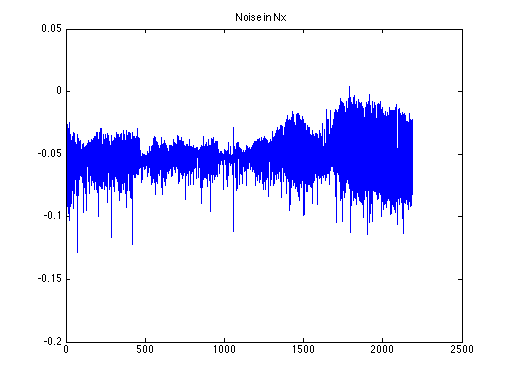
\includegraphics[width=0.45\textwidth]{noiseNx.PNG}
	}
	\;
	\subfloat[Ny]{
		\label{fig:errorNy}
		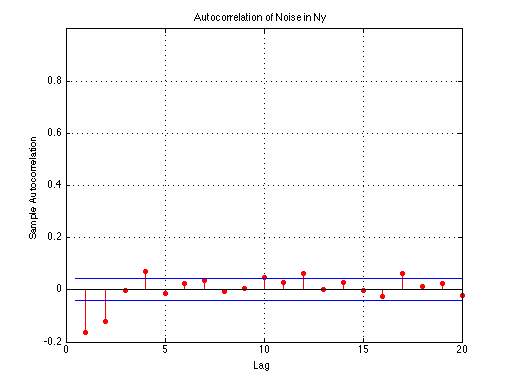
\includegraphics[width=0.45\textwidth]{noiseNy.PNG}
	}
	\;
	\subfloat[Nz]{
		\label{fig:errorNz}
		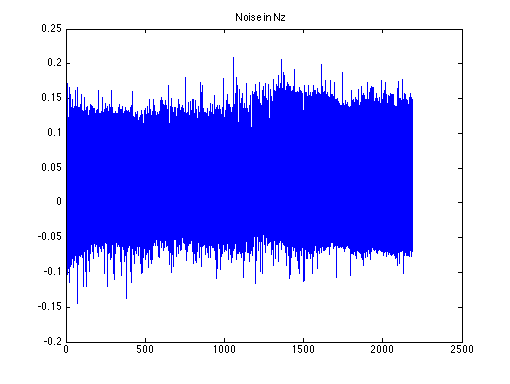
\includegraphics[width=0.45\textwidth]{noiseNz.PNG}
	}
	\;
	\subfloat[D]{
		\label{fig:errorD}
		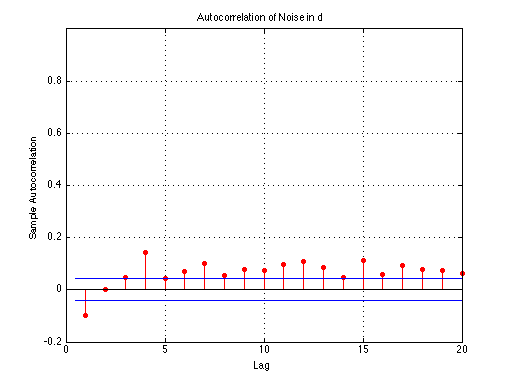
\includegraphics[width=0.45\textwidth]{noised.PNG}
	}
	\;
	\caption{Autocorrelation of error in innovation showing whiteness except for the distance variable}
	\label{fig:errorfigures}
\end{figure}


In order to verify that our system works with the kalman tuning, we ran it from our default initial position leaving it stationary. Below is the trajectory results. It shows a point cloud indicating that our kalman filter does indeed converge to some estimate of our real position fluctuating by only millimetres. This somewhat accurate result is due to the full observability provided by the three orthogonal planes lying in the xy, yz, zx spaces.


\begin{figure}[H]
	\begin{center}
		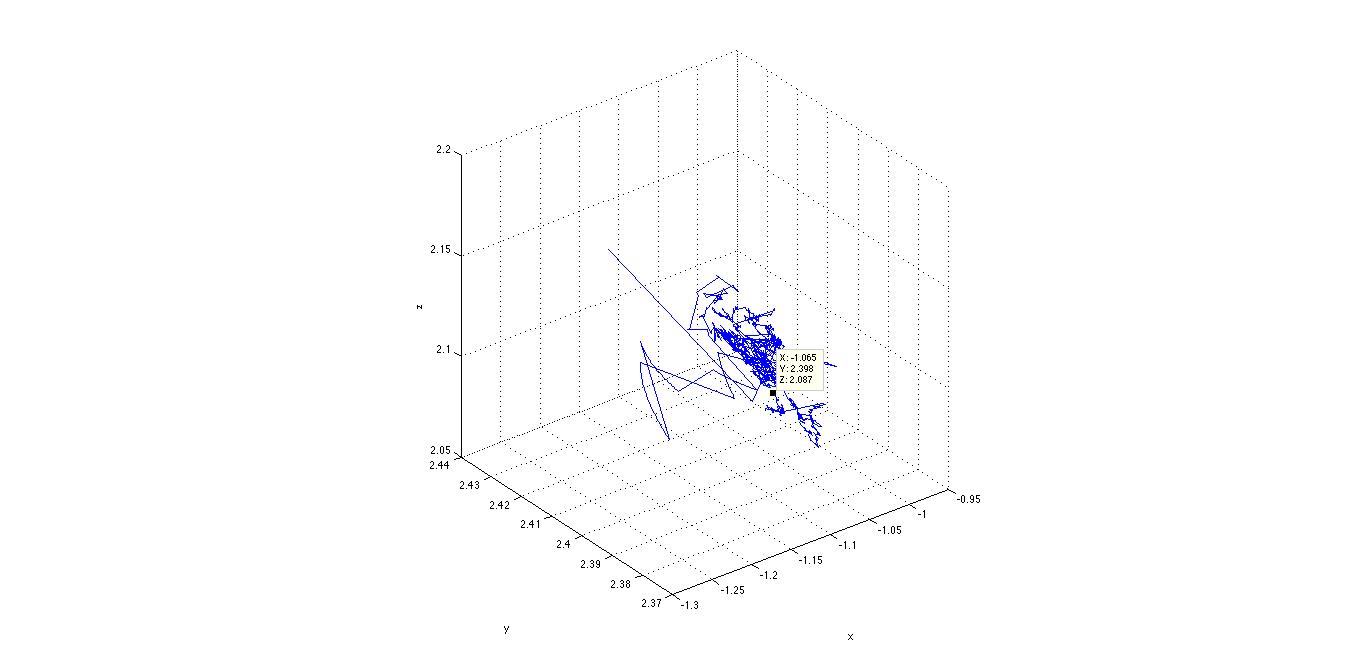
\includegraphics[width = \textwidth]{stationaryTraj.png}
	\end{center}
	\caption{Cloud point showing bounded Kalman filter stationary trajectory estimation}
	\label{fig:stationary_trajectory}
\end{figure}
In the second test, we moved the setup by hand in a pseudo straight line of length 1m along across on a table in the y axis whilst ensuring that three orthogonal planes are always observed. In the figure, we see that the variation in the z axis is small as the table provided low variation in the z axis. Also, fluctuations in state estimate are in the order of millimetres.

\begin{figure}[tbh]
	\subfloat[Using an Xtion factor of 10000] {
		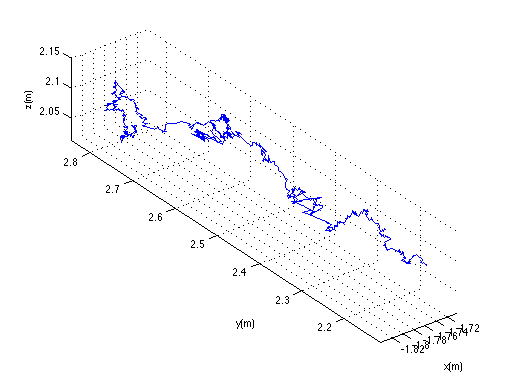
\includegraphics[width = \textwidth/2]{movingTraj.png}
	}
	\subfloat[Using an Xtion factor of 100(Higher frequency in estimation)] {
		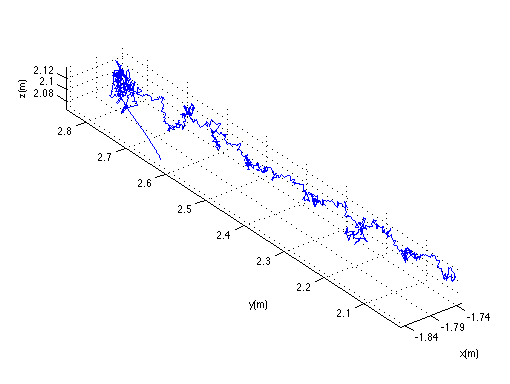
\includegraphics[width = \textwidth/2]{movingTraj100.png}
		\label{fig:trustXtion}
	}
	\caption{Cloud point showing bounded Kalman filter moving trajectory estimation over a distance of 1m in the y axis}
	\label{fig:moving_trajectory}
\end{figure}

To test the system on the quadcopter, it was decided to automate the yaw control. A yaw control loop was built where the system uses the estimated state to control the quad copter's yaw such that the depth camera (and hence frame of the craft) is always pointing towards a set point in the global coordinate system. The system was tested under lab conditions, where two intersecting planes were constructed to be used as a features for the system to localise against. Before flight the system was initialised to a known location, with the planes well within the depth camera's field of view. The quad copter was controlled remotely, and flown into a stable position out of ground effect before manually switching control of the yaw component to the automated control loop. So that the system doesn't lose visibility of the planes, the chosen point to track was the corner between the two constructed planes and the floor. 

%sentences 2 and 3 could be redundant
With the yaw control loop activated, it is obvious that the craft attempts to correct for yaw. However, the craft is required to be flown at a slow speed with gradual changes in position. Sudden movements or high speeds cause the craft to veer off in the direction of correction. Despite modifying the control loop parameters, rapid movement of the craft while in flight results in the system over compensating for yaw, over rotating the craft and then losing visibility. When visibility of both planes is lost for a short period of time, the Kalman filter relies more heavily upon the inertial sensors which are simply not accurate enough to obtain a good state estimate. Hence, the system ends up predicting an incorrect state, incorrectly attempts to correct the yaw and has to be grounded to prevent a collision. 


\section{Conclusion}
An off the shelf depth camera designed to track body movements (and hence had no need for precise distance measurements) was successfully calibrated using a custom calibration method. After this the point clouds generated gave accurate values and a distortion free image. This was instrumental for the detection of planes to work reliably. 

Selection of an appropriate computing platform was preformed, and showed that support for the ARM application processors and the software tools that we were using was not mature, and implementation was not tenable in the time frame. The final implementation used an x86 mini-itx board, which worked successfully but was sub optimal for weight and for connectivity to custom peripherals (specifically SPI).

A system was developed that correctly estimates the indoor state of a small aerial vehicle using an inexpensive and readily available depth camera coupled with an embedded platform. The state includes information about the quad copter such as position within the global coordinate system, velocity and attitude of the craft (yaw, pitch and roll). By using a Kalman filter which combines inertial sensors with a vision landmark map, an accuracy to within 10mm was achieved up to a distance of 4 meters. The vision system performed consistently well with minimal tuning and when paired with the Kalman filter, provided robust state estimation.


REGISTRATION

When mounted on an airframe the implementation successfully controled the yaw of the craft successfully, though the response was slow due to over correction. It has been hypothesised that the reason for the over correction in yaw at higher speeds is due to latency in the communication between the x86 platform and the R10 quad copter flight controller hardware. The slow communication was due to having to buffer the communication to the control board as there was not an SPI port available on the x86 board.

% The flight controller board only supports quad copter maneuverability control over a SPI bus, while the x86 board, which ran the vision and Kalman filter had no such interface. To enable communication between the two pieces of hardware, a small embedded processor known as an MBed was used. This processor ran a software SPI to USB bridge, allowing the x86 to connect to the flight controller through a USB port. The communication buffers in this bridge, the flight controller and the USB controller of the x86 board would amount to a considerable delay. From observing filmed footage of the craft in flight running the yaw control loop, the estimate for the latency between an the flight controller measuring the inertial sensors and the measurement being available for computation in the Linux environment is about half a second. This figure has not yet been confirmed or fully investigated, but would explain why the system cannot track the corner point at high speeds.

%Ryan would want to look at this
% An immediate solution to this problem is to use a platform with a dedicated SPI bus or install a fast peripheral SPI expansion card. If possible, decreasing the buffer size of both SPI and USB will reduce latency. Additionally, by using an RGB-D camera with a wider field of view should allow the system to maintain vision for longer. Further, using a smaller convolution kernel for normal estimation would allow more of the RGB-D image to be utilised. Another possibility is to use more accurate gyroscopes and accelerometers as when vision is lost, the system would take longer to lose state.   

\section{Further Work}
Although much work was done on trying to implement our system on an ARM application processor during the course of this project, significant problems surrounding compatibility with OpenNI (the frame work linking the Xtion depth camera with PCL). This is currently in version 1.6. Version 2.0 will be released soon and is intended to increase compatibility with arm platforms. This will allow a much lighter setup with more options of development boards with low level outputs, which would also solve some of the latency issues that we had. 

The algorithms described in this document would work much better if the inertial sensors were of high quality, as at the moment their noise causes the state estimate to diverge soon after observability of the planes is lost. Implementations utilising high quality sensors would yield more interesting results, as they could lose sight of previously registered planes and register new ones with an acceptable variance in their location to make full SLAM a possibility. 

There is also hope in the near future for consumer grade time of flight RGB-D camera to be widely available, due to these being used in the XBox One console. These will have less quantisation noise, and a much wider field of view. This would solve a number of issues that we had regarding losing sight of known planes before observing new ones to register, as well as removing much of the noise from the raw depth data. 




\clearpage

\nocite{*}

\printbibliography
% \bibliography{biblib}{}
% \bibliographystyle{plain}
% \begin{thebibliography}{99}

% \bibitem{todo}
% 	THIS REFERENCE IS MISSING!

% \bibitem{MARSlab}
% 	Nikolas Trawny and Stergios I. Roumeliotis,
% 	\emph{Indirect Kalman Filter for 3D Attitude Estimation, A Tutorial for Quaternion Algebra}. \\
% 	\url{http://www-users.cs.umn.edu/~trawny/Publications/Quaternions_3D.pdf}

% \bibitem{MATLABAerospace}
% 	MathWorks,
% 	\emph{Implement quaternion representation of six-degrees-of-freedom equations of motion with respect to body axes}. \\
% 	\url{http://www.mathworks.co.uk/help/aeroblks/6dofquaternion.html}

% \bibitem{OpenPilotPaper}
% 	Dale E. Schinstock,
% 	\emph{GPS-aided INS Solution for OpenPilot}. \\
% 	\url{http://wiki.openpilot.org/download/attachments/950387/INSGPSAlg.pdf}

% \bibitem{KFBookSerialupdate}
% 	Grewal, M.S., A.P. Andrews,
% 	\emph{Kalman Filtering, Theory and Practice Using MATLAB}. \\
% 	\url{http://www.control.aau.dk/~obin03/ESIF/Grewal,%20Andrews%20Kalman%20Filtering%20Theory%20And%20Practice%20Using%20Matlab%20(2Ed%20,%20Wiley,%202001)(410S).pdf}

% \bibitem{OpenPilotinsgps}
% 	The OpenPilot Team,
% 	\emph{Joint attitude and position estimation EKF}. \\
% 	\url{http://reviews.openpilot.org/browse/OpenPilot/flight/libraries/insgps16state.c?hb=true}

% \bibitem{ThirdYearControl}
% 	Alessandro Astolfi,
% 	\emph{Systems and Control Theory - An Introduction}. \\
% 	\url{http://www3.imperial.ac.uk/pls/portallive/docs/1/31851696.PDF}

% \bibitem{BerkelyCourse}
% 	Pieter Abbeel,
% 	\emph{Learning for robotics and control}. \\
% 	\url{http://inst.eecs.berkeley.edu/~cs294-40/fa08/#syllabus}

% \bibitem{HexCoptSelfCalb}%some interesting stuff about online sensor calibration. also quite embedded solution
% 	Stephan Weiss, Markus W. Achtelik, Margarita Chli, Roland Siegwart,
% 	\emph{Versatile Distributed Pose Estimation and Sensor
% 			Self-Calibration for an Autonomous MAV}. \\
% 	\url{http://ieeexplore.ieee.org/stamp/stamp.jsp?tp=&arnumber=6225002}

% \bibitem{KinectCopter}%very close to our solution, using kinect and atom. focus on navigation/exploration
% 	Shaojie Shen, Nathan Michael, and Vijay Kumar,
% 	\emph{Autonomous Indoor 3D Exploration with a Micro-Aerial Vehicle}. \\
% 	\url{http://ieeexplore.ieee.org/stamp/stamp.jsp?tp=&arnumber=6225146}

% \bibitem{AgresivePlane}%very close to our solution, using kinect and atom. focus on navigation/exploration
% 	Adam Bry, Abraham Bachrach, Nicholas Roy,
% 	\emph{State Estimation for Aggressive Flight in GPS-Denied Environments
% 			Using Onboard Sensing}. \\
% 	\url{http://ieeexplore.ieee.org/stamp/stamp.jsp?tp=&arnumber=6225295}

% \bibitem{CompareFilters}%Comparision between kalman and particle filter.
% Manya Afonso
% \emph{Particle Filter and Extended Kalman Filter for Nonlinear Estimation: A Comparative Study}.
%  \url{http://users.isr.ist.utl.pt/~pjcro/cadeiras/dsfps0708/SEMS/PF_EKF_TermPaper.pdf}
% \end{thebibliography}


\end{document}

